
%
% Chapter 8
%

\chapter{Results}
\epigraph{There are two possible outcomes: if the result confirms the hypothesis, then you've made a measurement. If the result is contrary to the hypothesis, then you've made a discovery.}{\textit{Enrico Fermi}}
\label{results}
In this chapter the results of both the searches are presented. The results for the $\hmue$ search are first presented. Results for the $\Hmue$ search follow.

\subsection{$\hmue$ results}
The resulting distributions of the signal variable (after applying all selection requirements as outlined in ~\ref{h125_evt_sel}) are fit using a binned maximum likelihood fit. The entire procedure is described in detail in ~\ref{stat_meth}. All systematic uncertainties are included as nuisance parameters, and the fit is performed simultaneously across all categories. The BDT response distributions of signal and background are shown superimposed for each category in Fig~\ref{fig:BDT_dist_hmue}. The distribution of $\mcol$ for the $\mcol$-fit analysis are also shown in Fig~\ref{fig:mcol_dist_hmue}. We do not observe an excess of signal over expected background. Hence, upper exclusion limits on $\mathcal{B}(\hmue)$ are set, following the procedure described in ~\ref{exc_cal}. In table~\ref{table:hmue_limits}, the median expected limits, observed limits and the best fit branching fractions for $\mathcal{B}(\hmue)$ are summarized. As noted earlier in this thesis, the tau lepton coming from the Higgs can also decay hadronically. This channel of the LFV Higgs decay, i.e. $\hmuhad$ is studied in an analyses by different members of the same research team~\cite{HIG-17-001}. The limits on $\mathcal{B}(\hmuhad)$ from that search are combined with limits on $\mathcal{B}(\hmue)$, as calculated above from the search described here. All limits are summarized graphically in Figure~\ref{fig:hmue_limits_brazil}. The combined observed (median expected) upper limits on $\mathcal{B}(\hmu)$ is 0.25 (0.25)\,\% at 95\% CL, for the BDT-fit analysis. The combined best fit branching fraction of $\mathcal{B}(\hmu)$ is found to be $0.00 \pm 0.12$, also for the BDT-fit analysis. It is important to note that the 2.4\,$\sigma$ excess observed by the earlier CMS search with 8 TeV data~\cite{Khachatryan:2015kon} has now been excluded by this search.


\begin{table*}[!htpb]
 \begin{center}
   \caption{Expected and observed upper limits at 95\% CL, and best fit branching fractions in percent for each individual jet category, and combined, for the $\hmue$ analysis.}
   \scalebox{0.85}{
\begin{tabular}{*{6}{c}}
\multicolumn{6}{c}{Expected limits~(\%) } \\ \hline
                       &  \multicolumn{1}{c}{0-jet}   & \multicolumn{1}{c}{1-jet}    &  \multicolumn{1}{c}{2-jets} & \multicolumn{1}{c}{VBF}  & \multicolumn{1}{c}{Combined}                 \\  \cline{2-6}
BDT fit analysis 	 &  $<$0.83   	 &  $<$1.19   	 &  $<$1.98   	 &  $<$1.62   	 &  $<$0.59    \\
$\mcol$ fit analysis 	 &  $<$1.01   	 &  $<$1.47   	 &  $<$3.23   	 &  $<$1.73   	 &  $<$0.75    \\
\cline{2-6}
\\ [\cmsTabSkip]
\multicolumn{6}{c}{Observed limits~(\%)} \\ \hline
                       &  \multicolumn{1}{c}{0-jet}   & \multicolumn{1}{c}{1-jet}    &  \multicolumn{1}{c}{2-jets} & \multicolumn{1}{c}{VBF} &\multicolumn{1}{c}{Combined}                 \\ \cline{2-6}
BDT fit analysis   		 & $<$1.30   	 & $<$1.34   	 & $<$2.27   	 & $<$1.79   	 & $<$0.86    \\
$\mcol$ fit analysis   		 & $<$1.08   	 & $<$1.35   	 & $<$3.33   	 & $<$1.40   	 & $<$0.71    \\
\cline{2-6}
\\[\cmsTabSkip]
\multicolumn{6}{c}{Best fit branching fractions~(\%)} \\ \hline
                       &  \multicolumn{1}{c}{0-jet}   & \multicolumn{1}{c}{1-jet}    &  \multicolumn{1}{c}{2-jets} & \multicolumn{1}{c}{VBF} &\multicolumn{1}{c}{Combined}                 \\  \cline{2-6}
BDT fit analysis    		 & 0.61 $\pm$ 0.36  	 & 0.22 $\pm$ 0.46  	 & 0.39 $\pm$ 0.83  	 & 0.10 $\pm$ 1.37  	 & 0.35 $\pm$ 0.26  \\
$\mcol$ fit analysis    		 & 0.13 $\pm$ 0.43  	 & $-0.22$ $\pm$ 0.75  	 & 0.22 $\pm$ 1.39  	 & $-1.73$ $\pm$ 1.05  	 & $-0.04$ $\pm$ 0.33  \\
\cline{2-6}
combined $\Pgm\Pgt$ (BDT fit)  & \multicolumn{5}{c}{ 0.00 $\pm$ 0.12 } \\ \hline
\end{tabular}}
\end{center}
\label{table:hmue_limits}
\end{table*}

\begin{figure*}[!htpb]\centering
 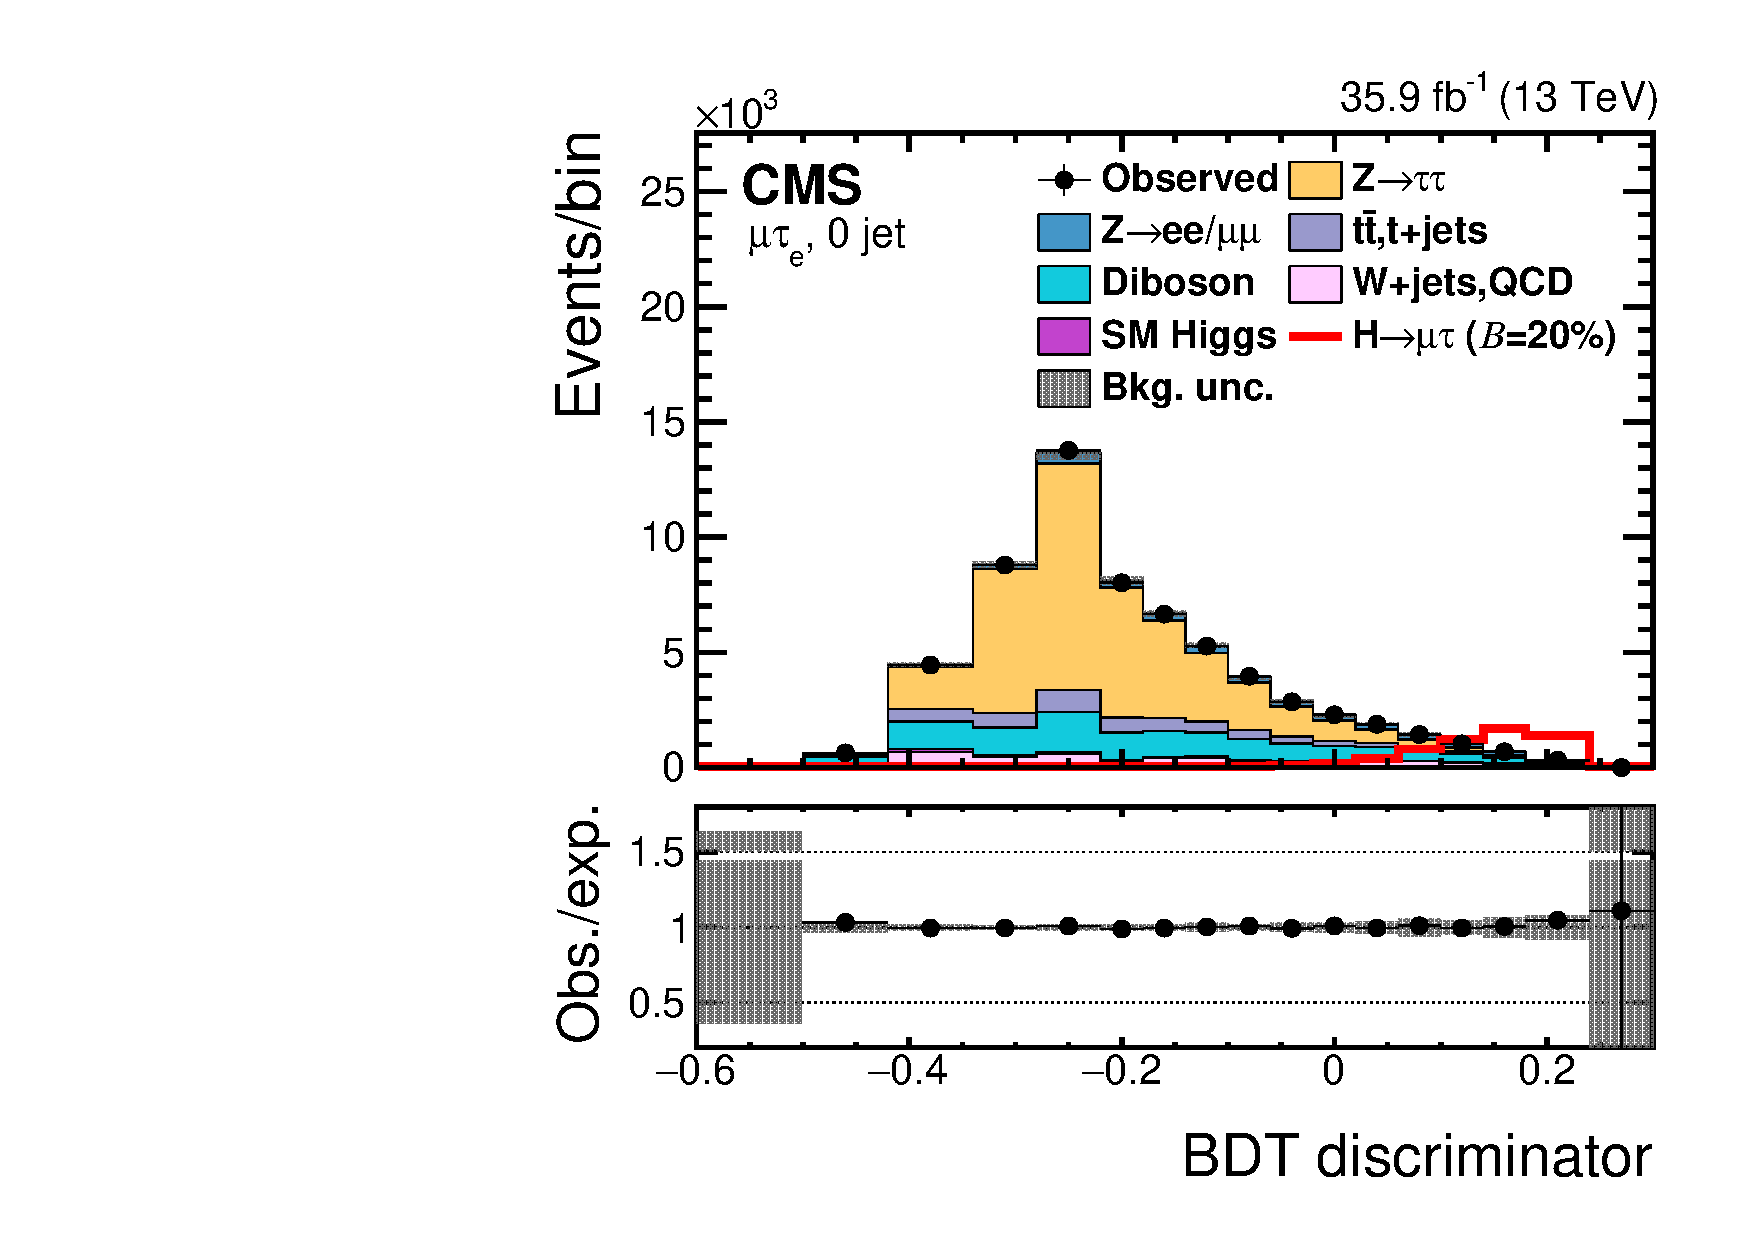
\includegraphics[width=0.49\textwidth]{plots_and_figures/chapter8/h125/0jetBDT.pdf}
 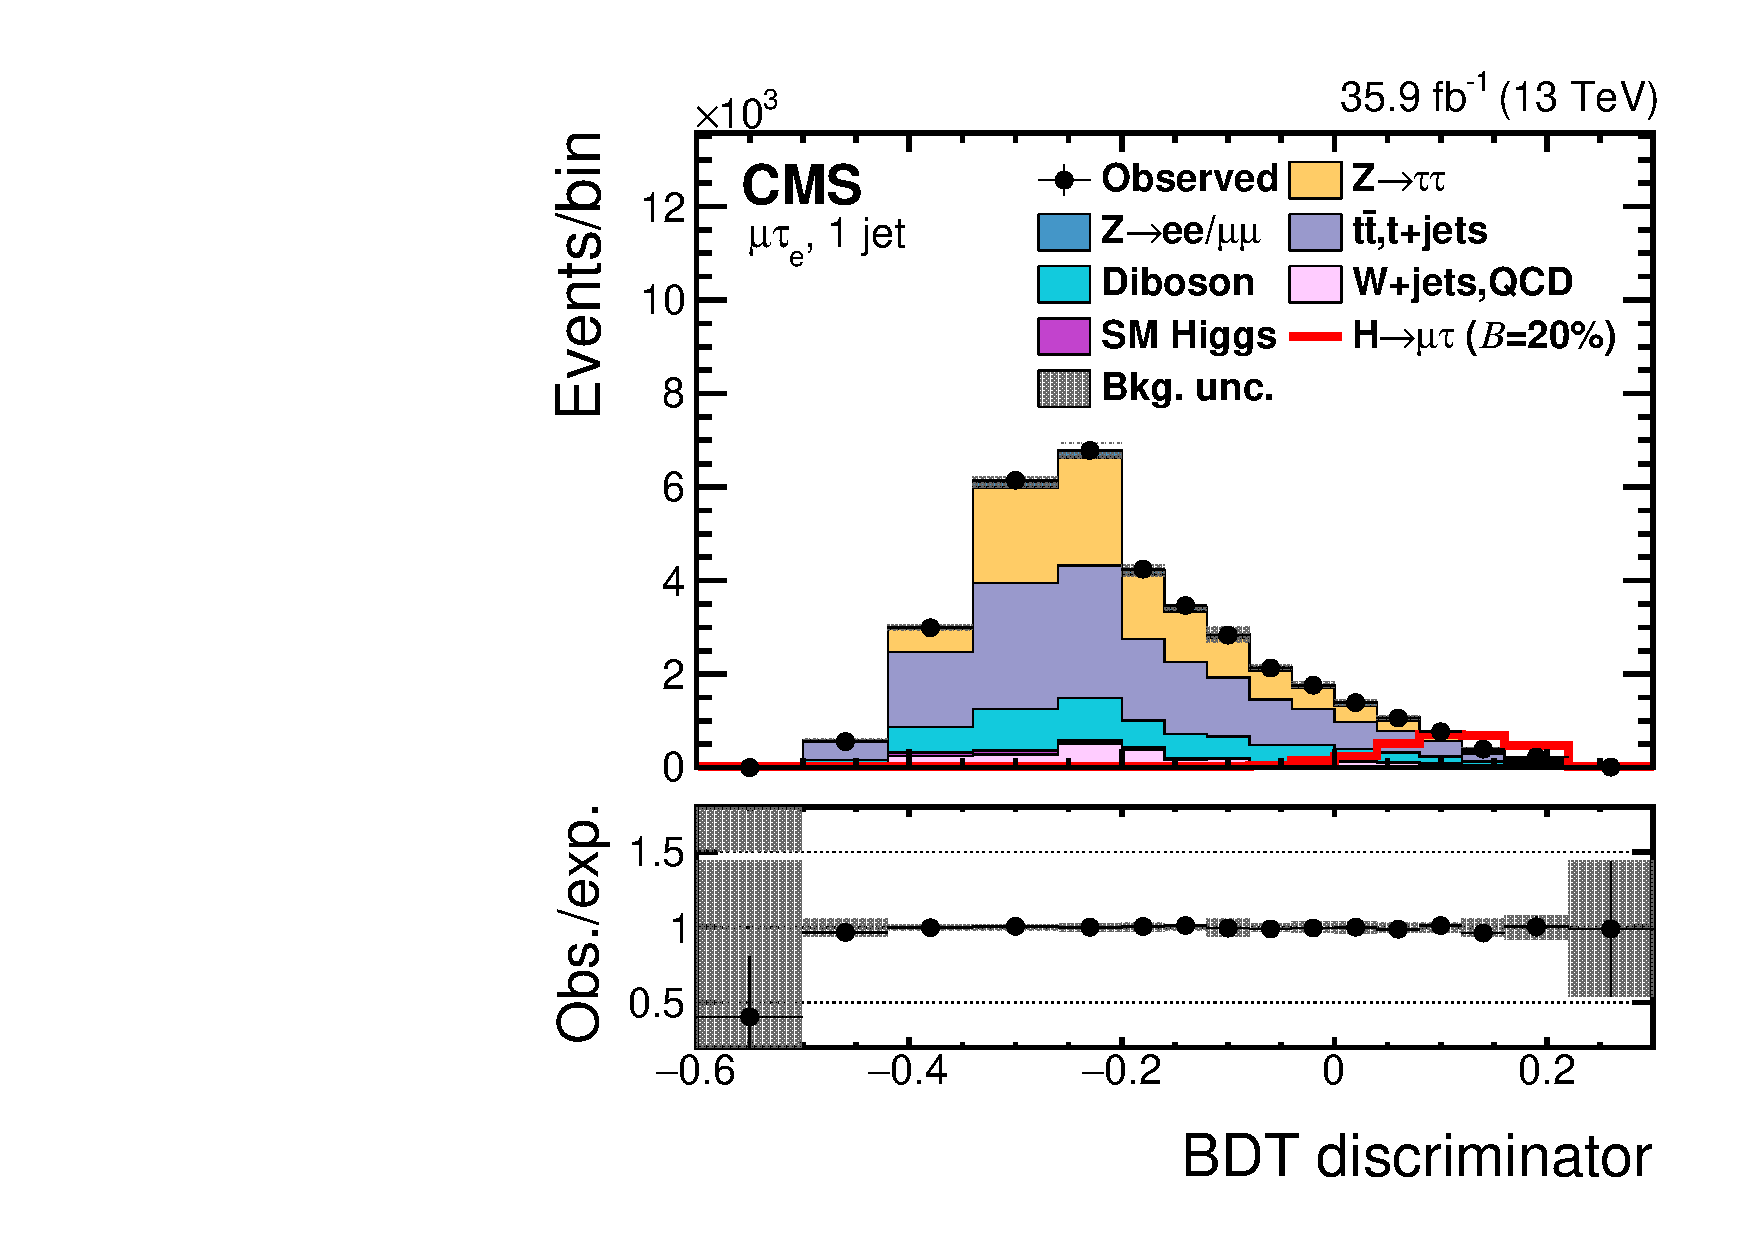
\includegraphics[width=0.49\textwidth]{plots_and_figures/chapter8/h125/1jetBDT.pdf} \\
 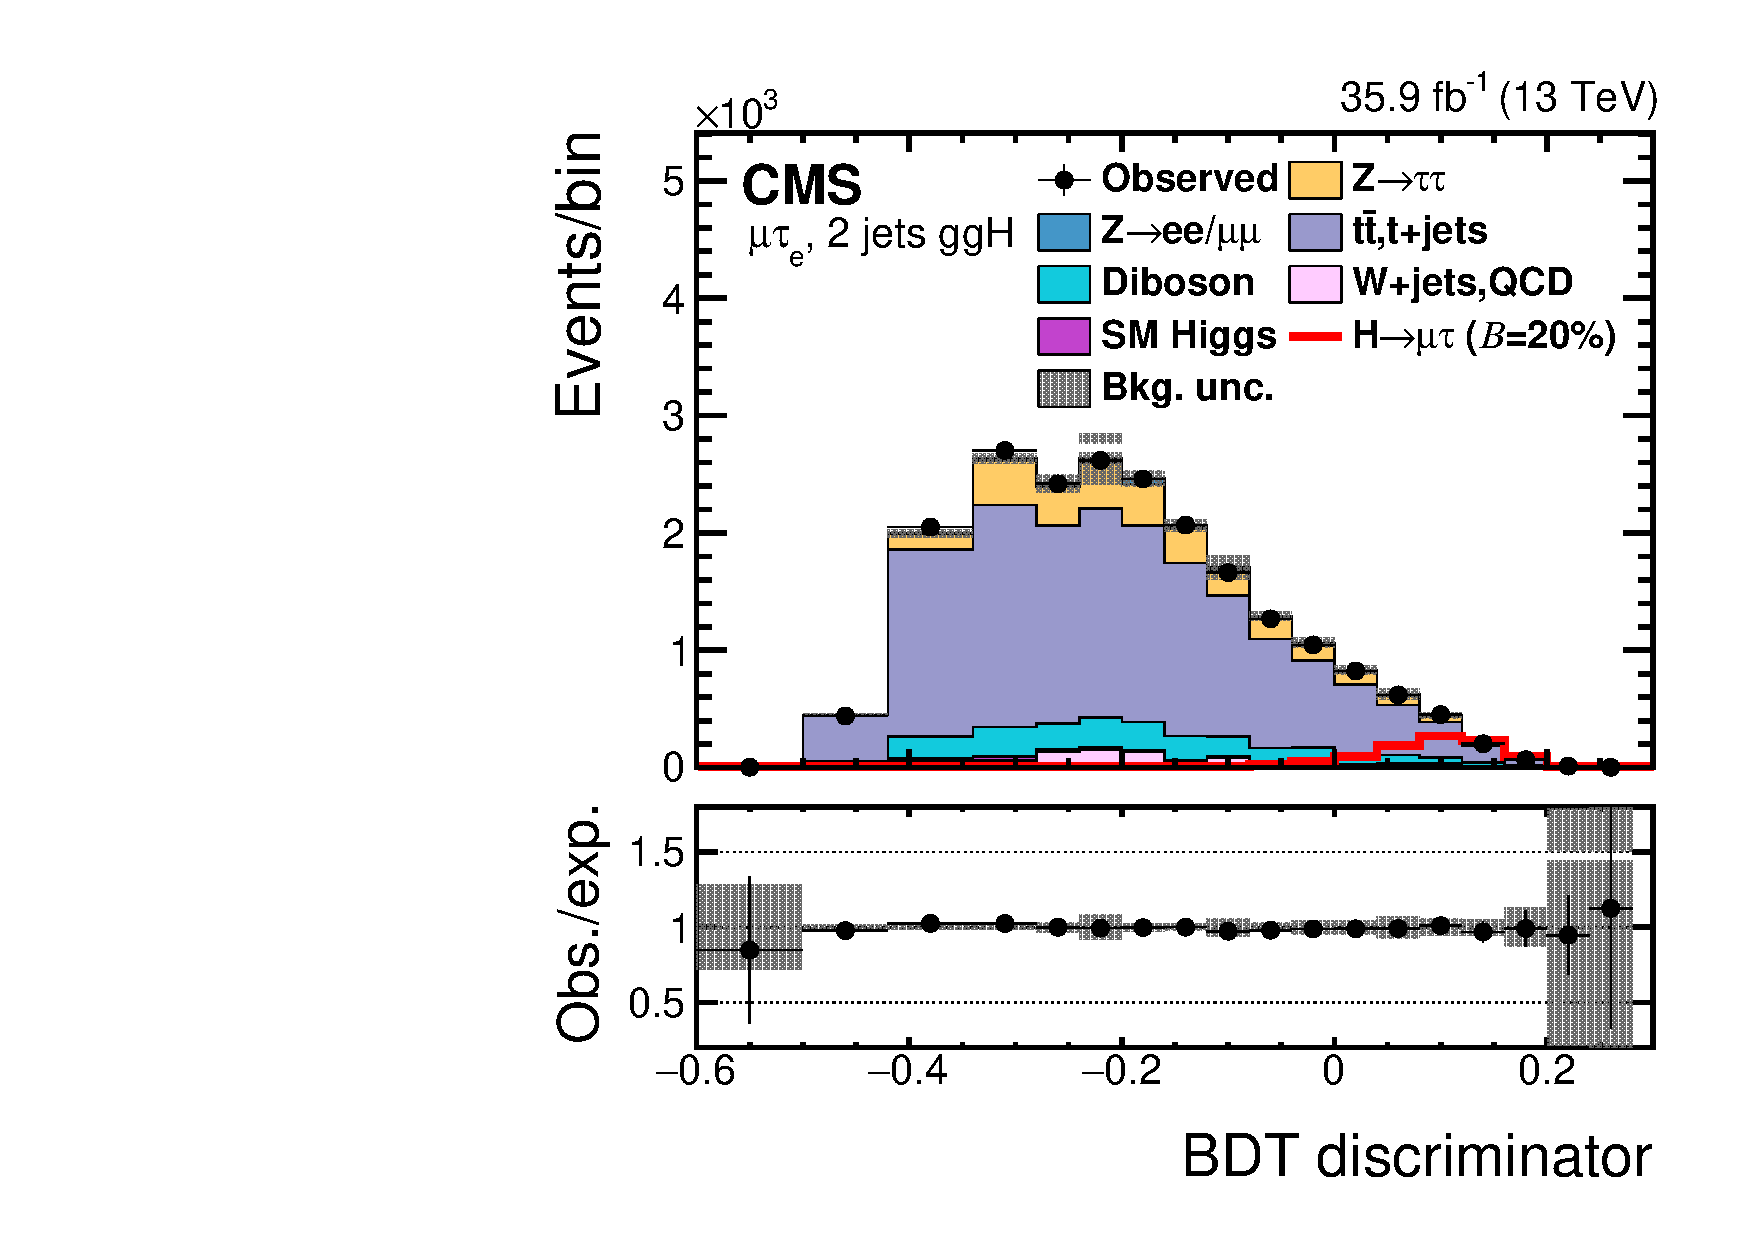
\includegraphics[width=0.49\textwidth]{plots_and_figures/chapter8/h125/2jetggBDT.pdf}
 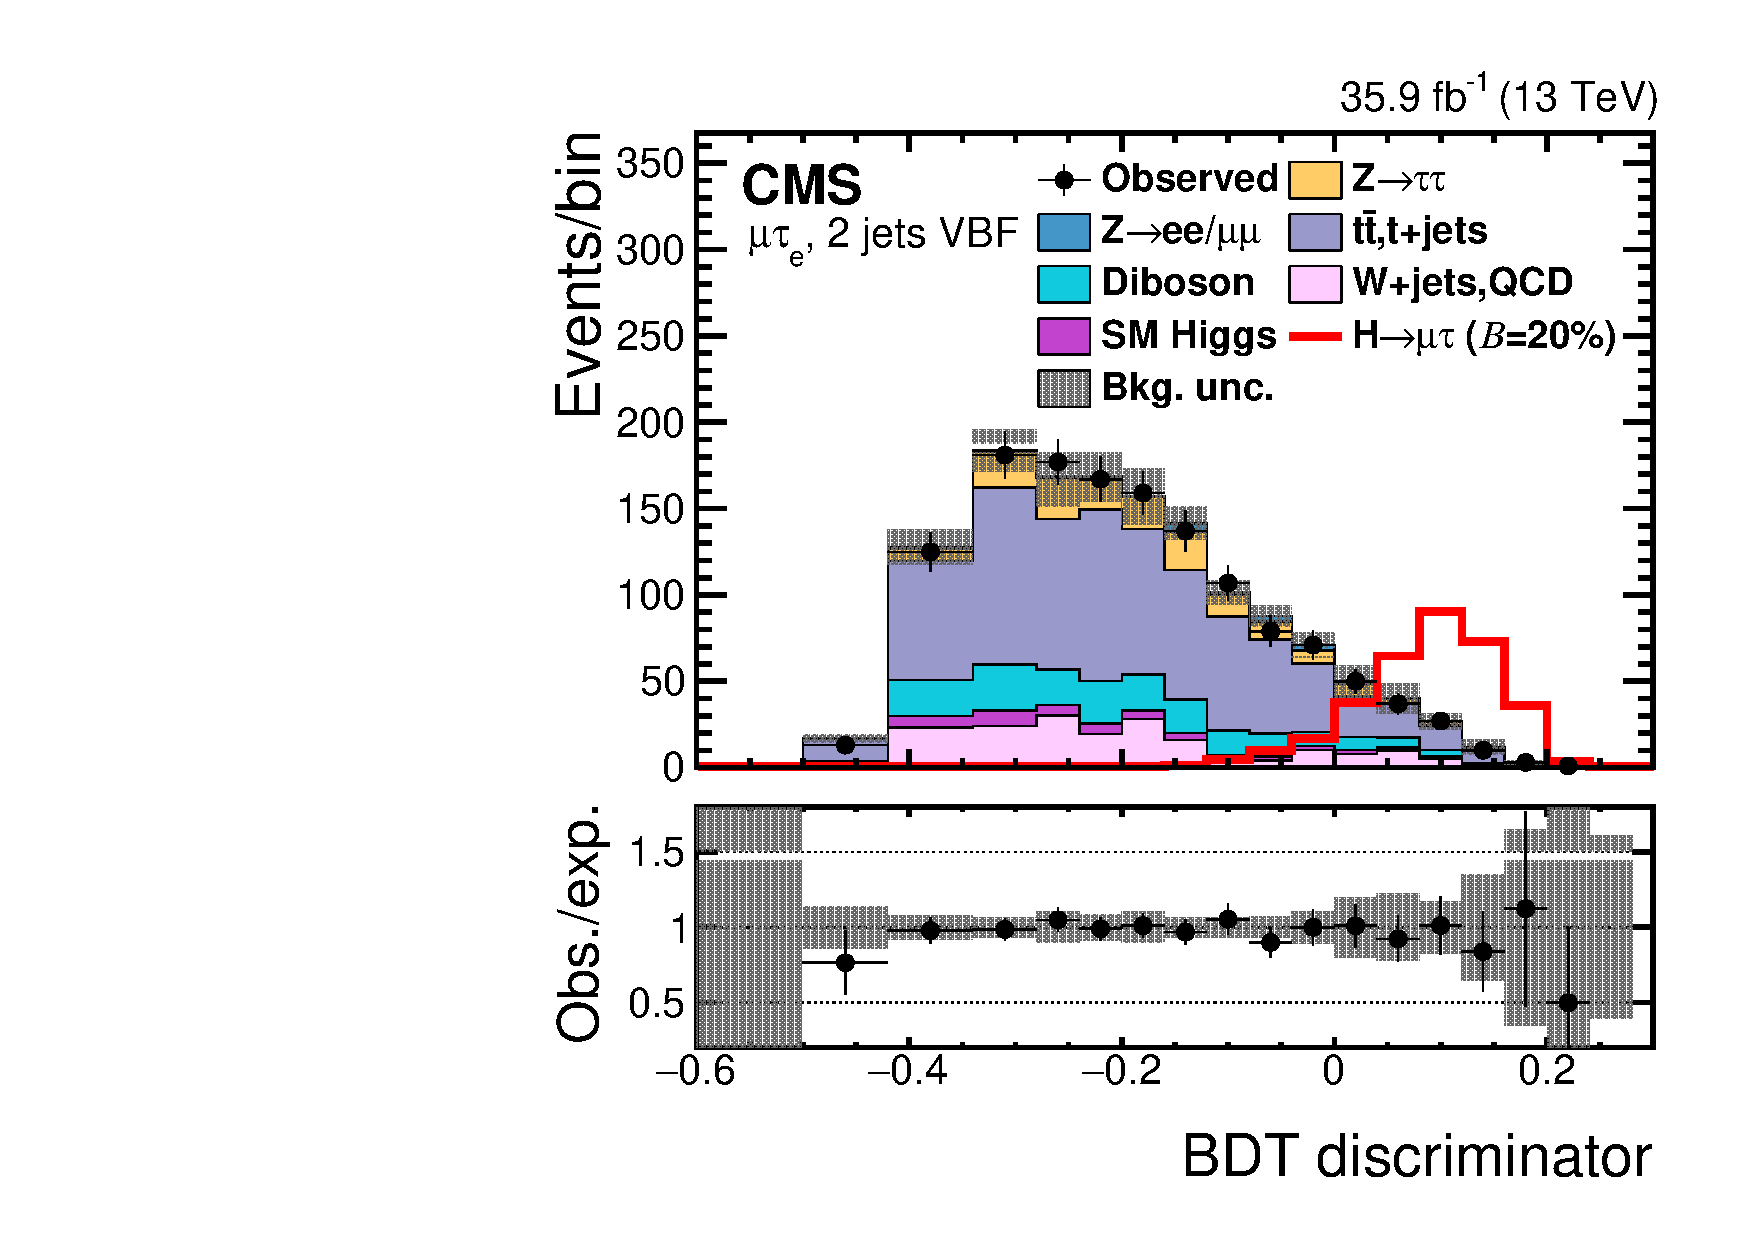
\includegraphics[width=0.49\textwidth]{plots_and_figures/chapter8/h125/2jetvbBDT.pdf} 
\caption{Distribution of BDT response in each category comparing signal and background estimations to observed collision data, for $\hmue$ analysis. The bottom panel show the ratio of observed data and fitted background in each bin~\cite{HIG-17-001}}
 \label{fig:BDT_dist_hmue}
\end{figure*}

\begin{figure*}[!htpb]\centering
 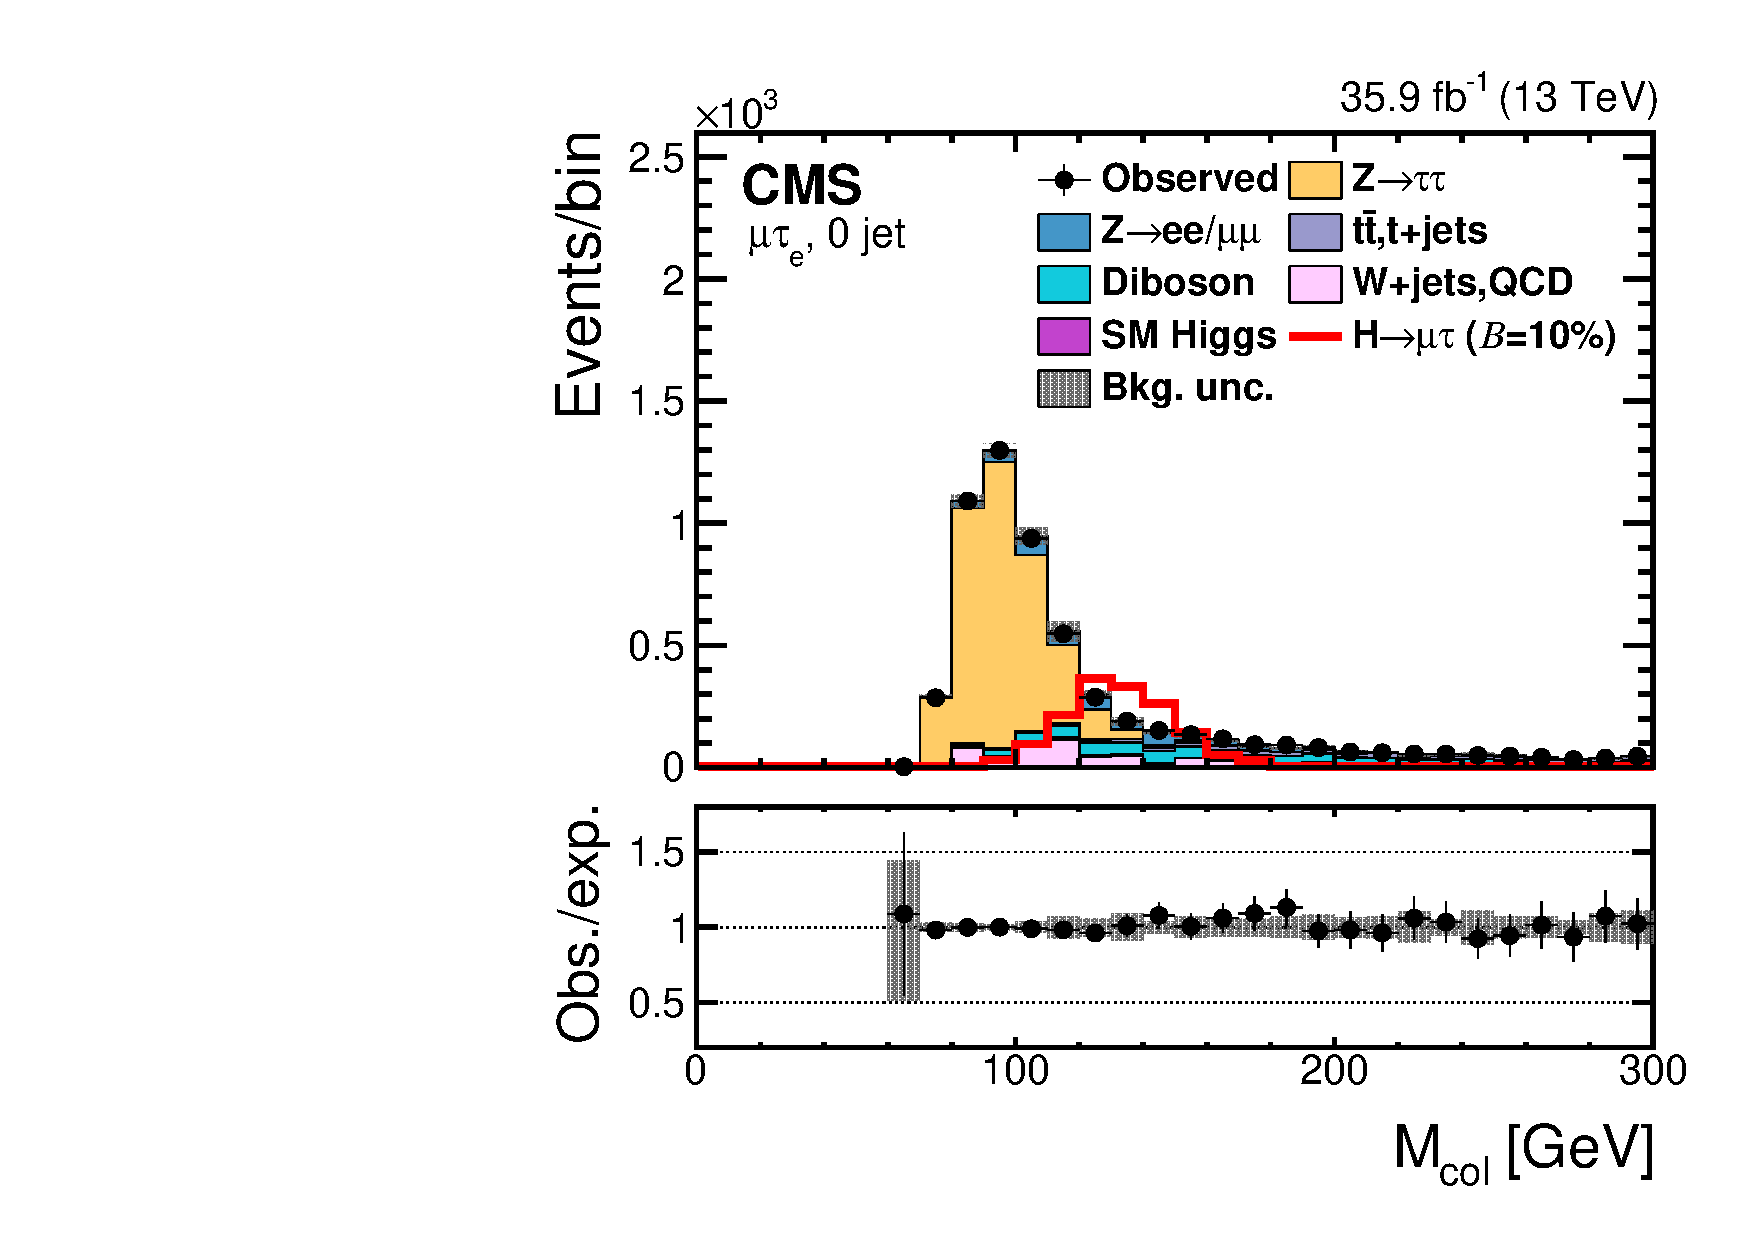
\includegraphics[width=0.49\textwidth]{plots_and_figures/chapter8/h125/0jetmcol.pdf}
 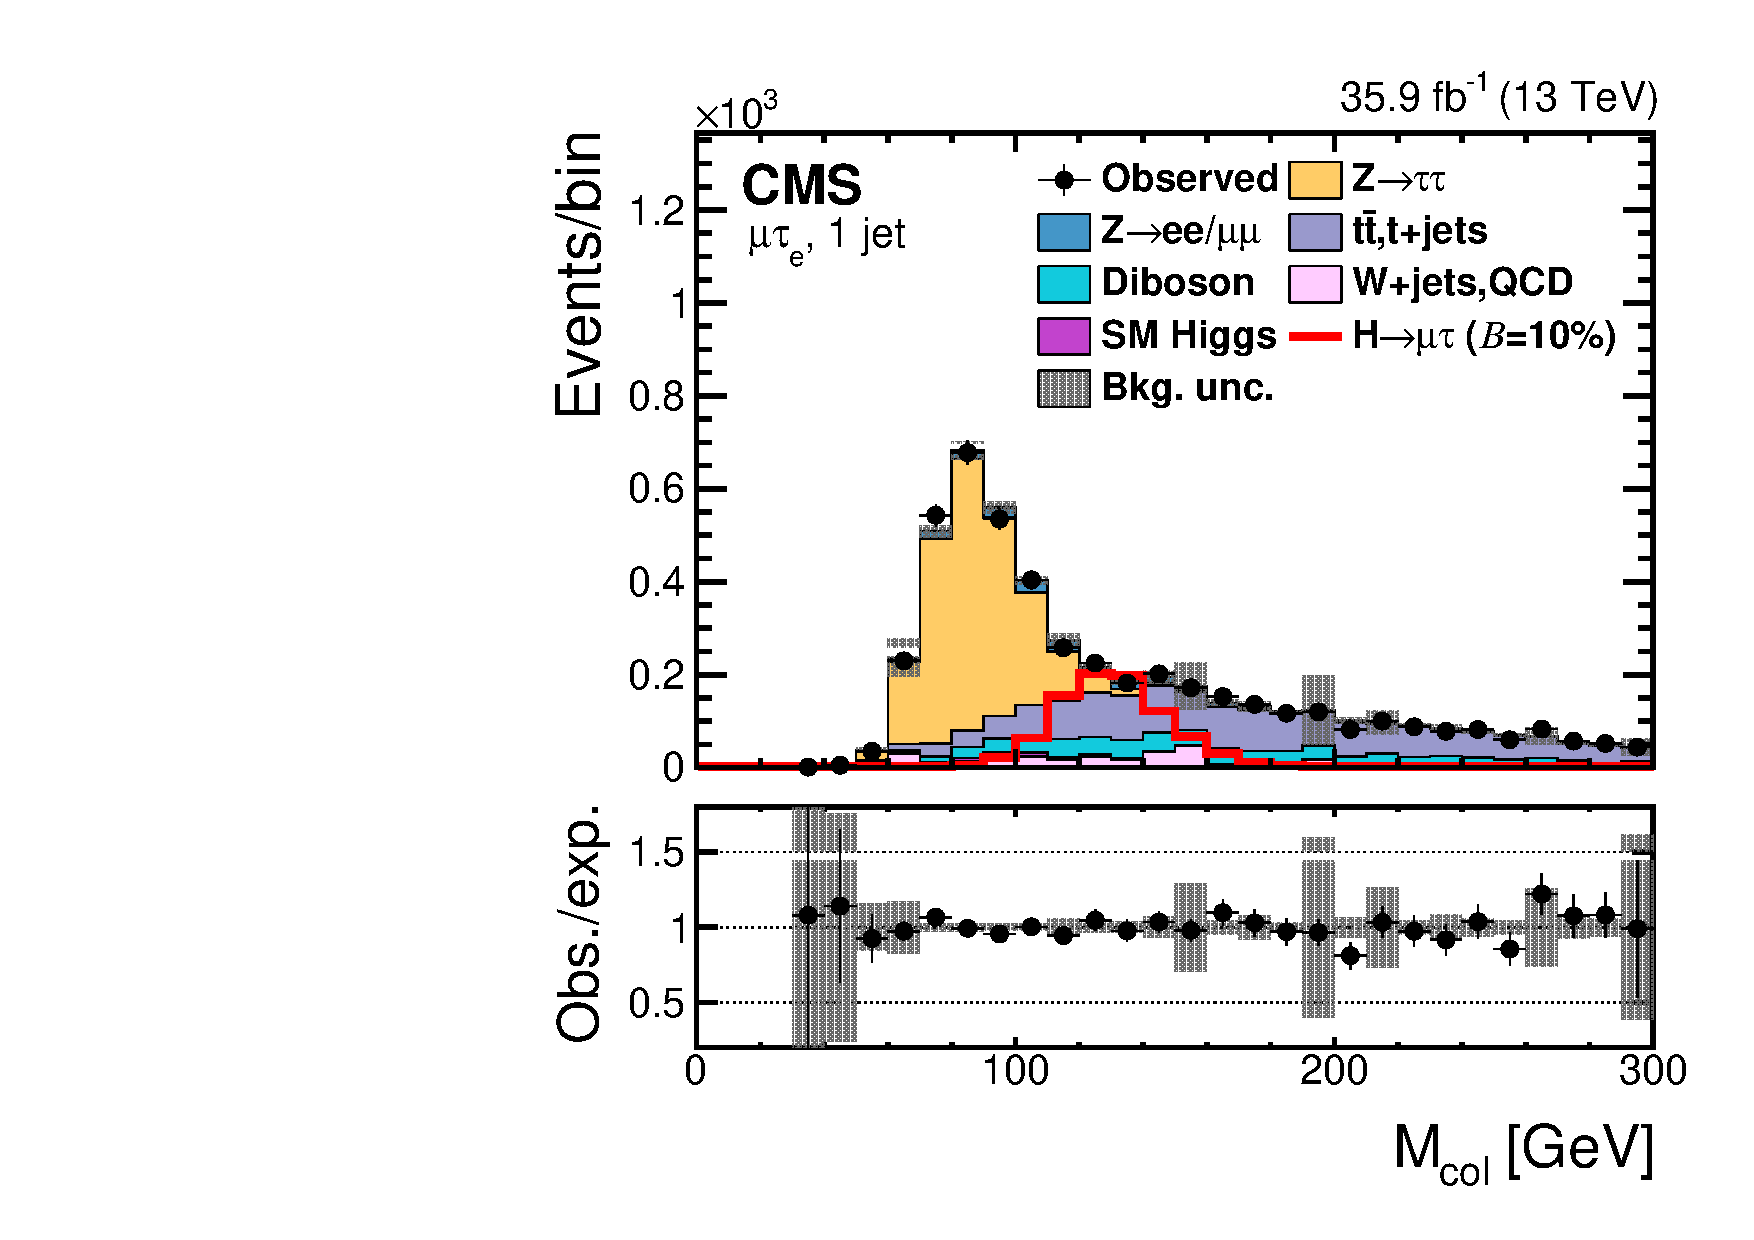
\includegraphics[width=0.49\textwidth]{plots_and_figures/chapter8/h125/1jetmcol.pdf} \\
 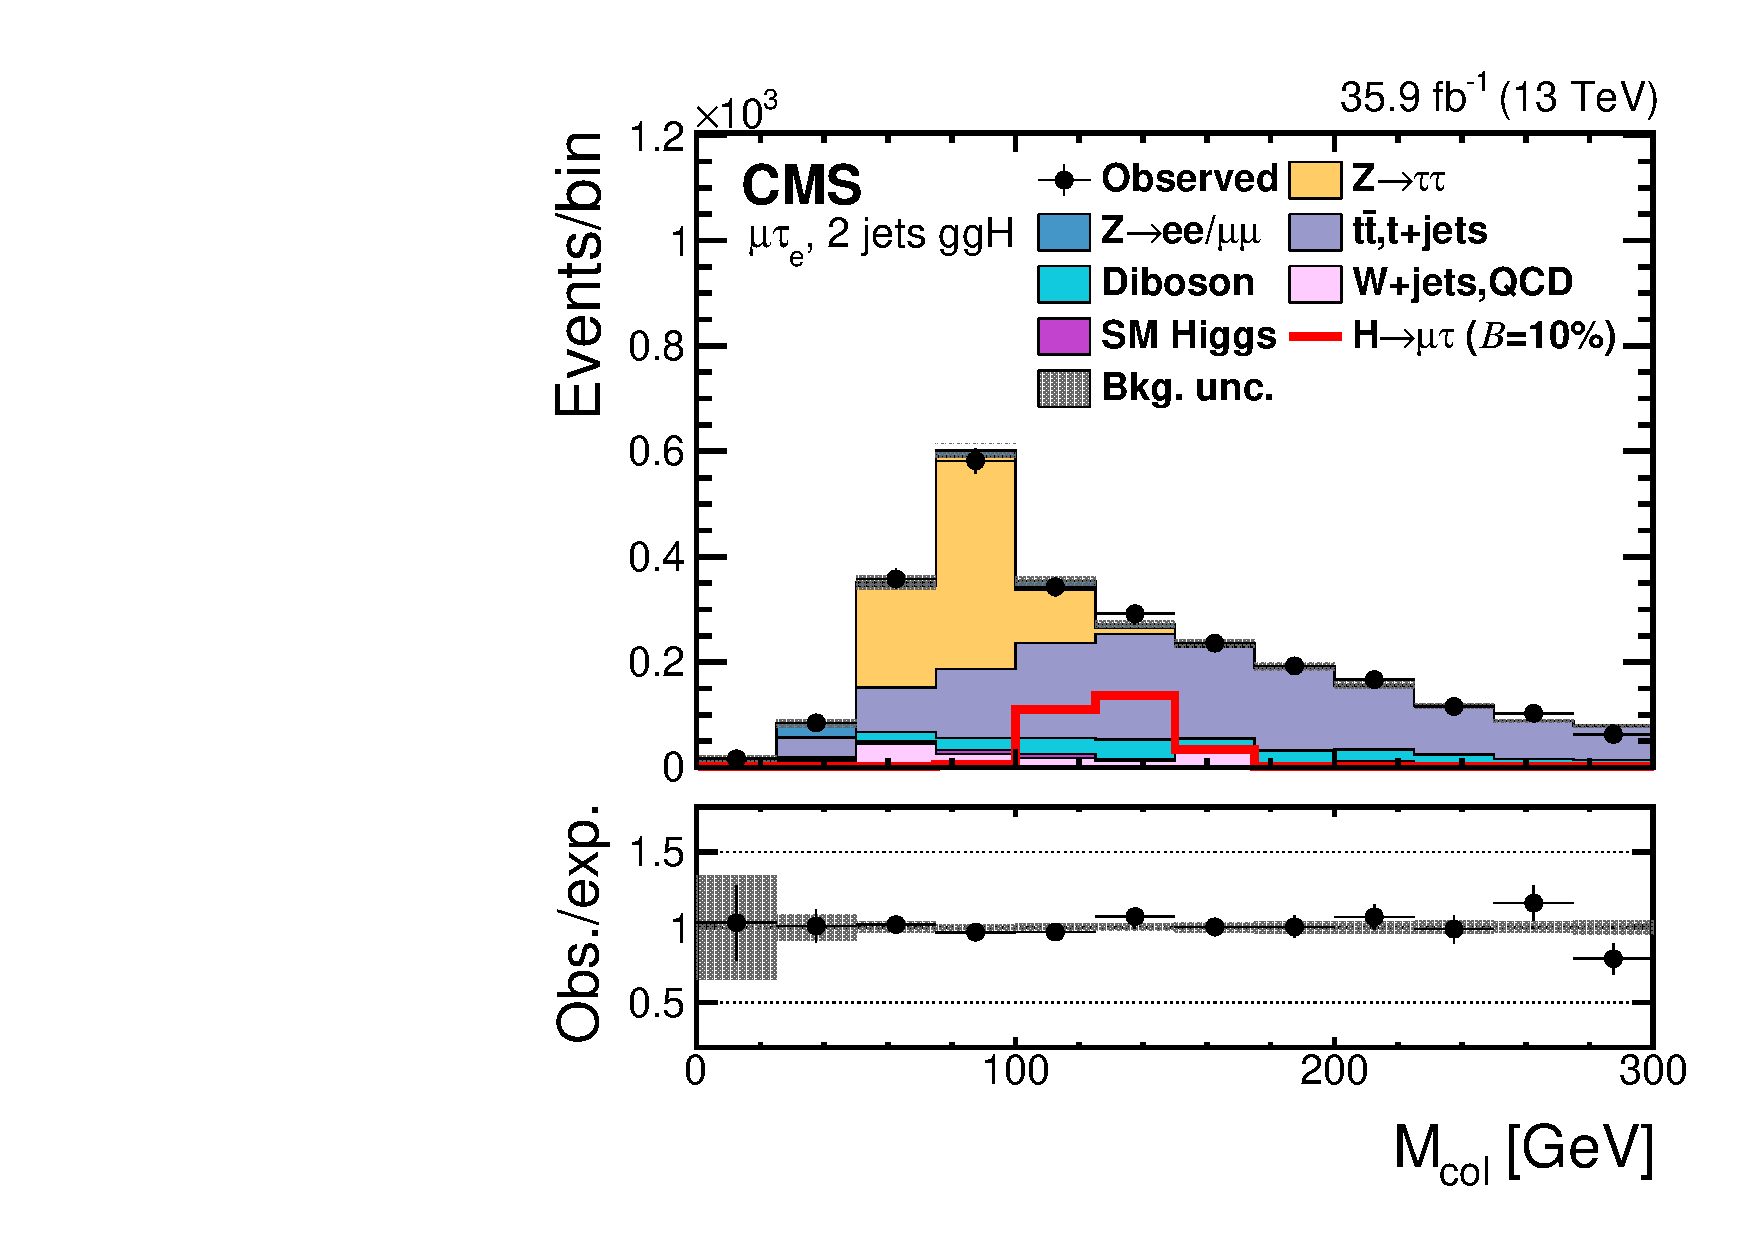
\includegraphics[width=0.49\textwidth]{plots_and_figures/chapter8/h125/2jetggmcol.pdf}
 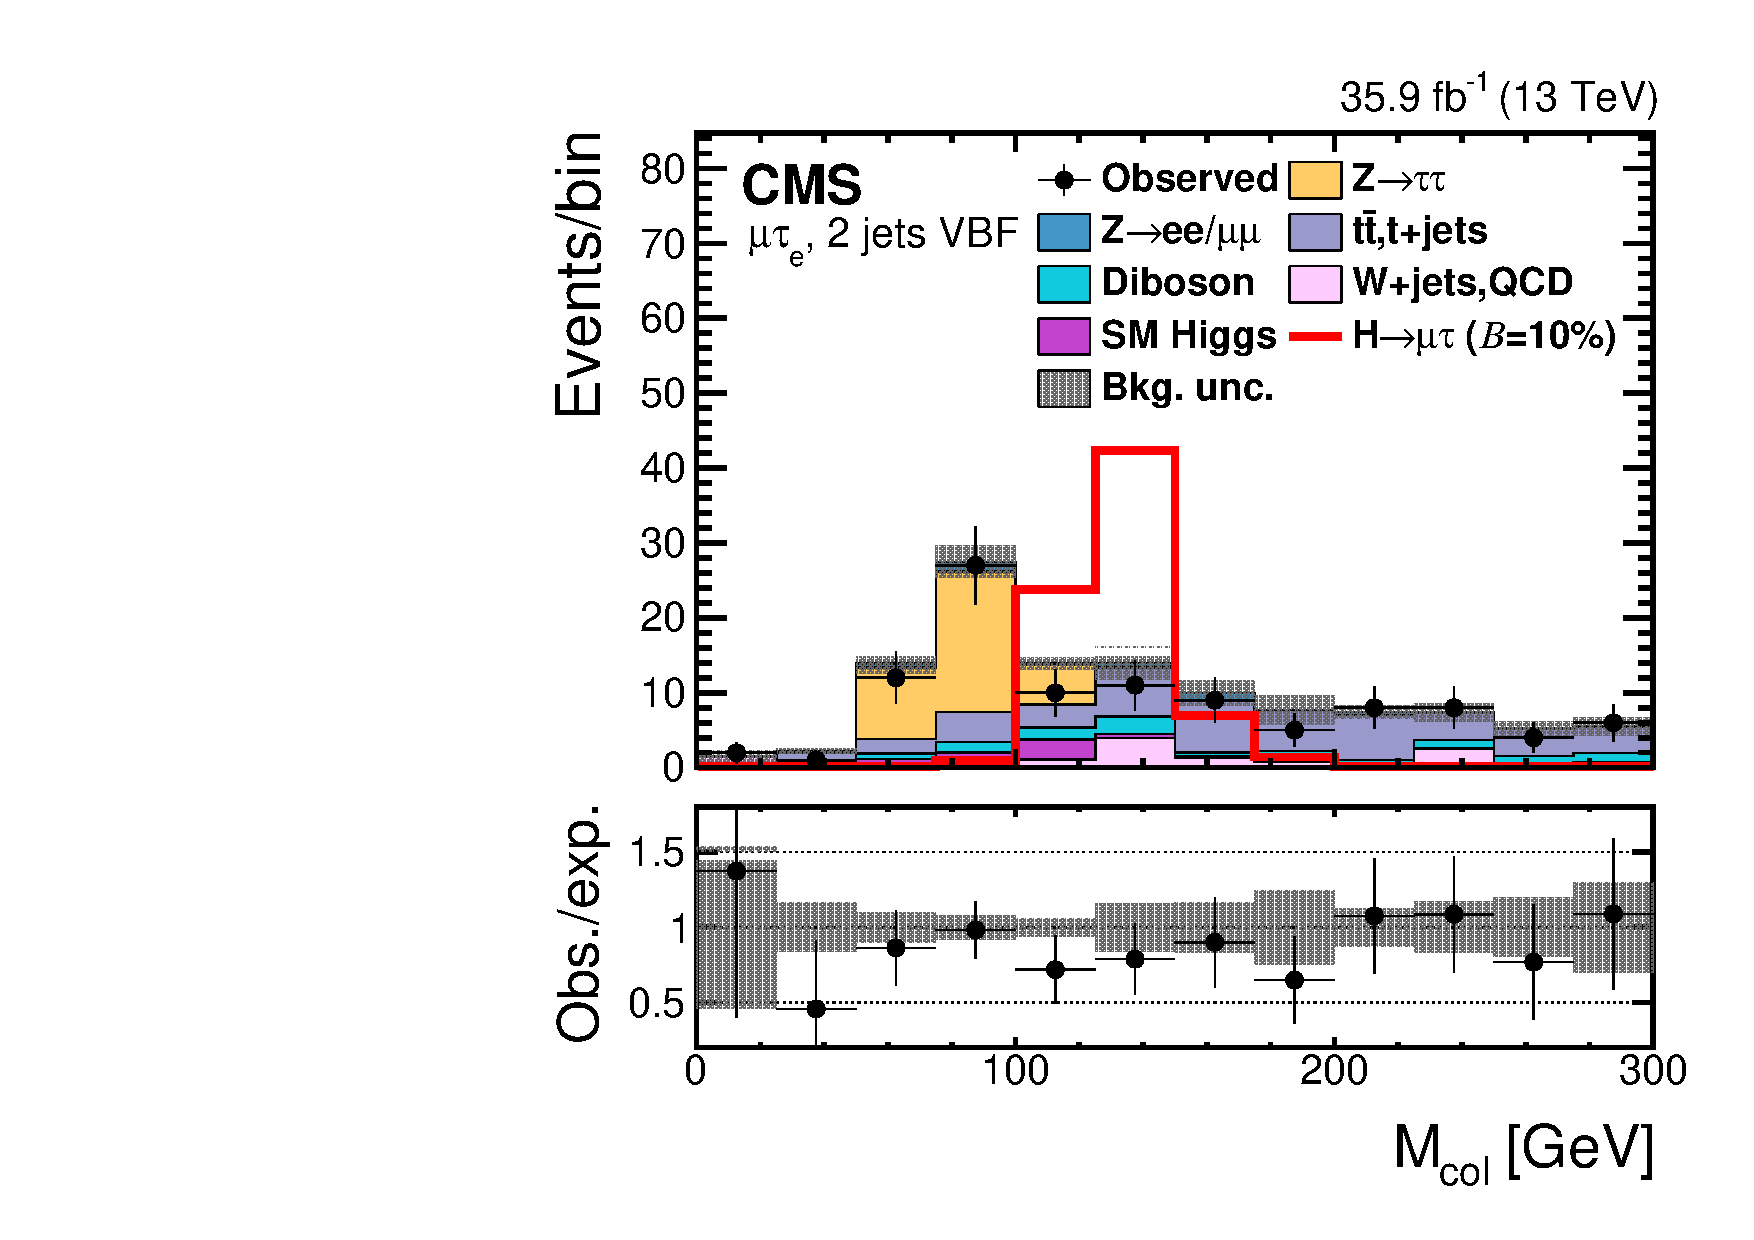
\includegraphics[width=0.49\textwidth]{plots_and_figures/chapter8/h125/2jetvbmcol.pdf} 
\caption{Distribution of $\mcol$ response in each category comparing signal and background estimations to observed collision data, for $\hmue$ analysis. The bottom panel show the ratio of observed data and fitted background in each bin~\cite{HIG-17-001}}
 \label{fig:mcol_dist_hmue}
\end{figure*}

\begin{figure*}[!htpb]\centering
 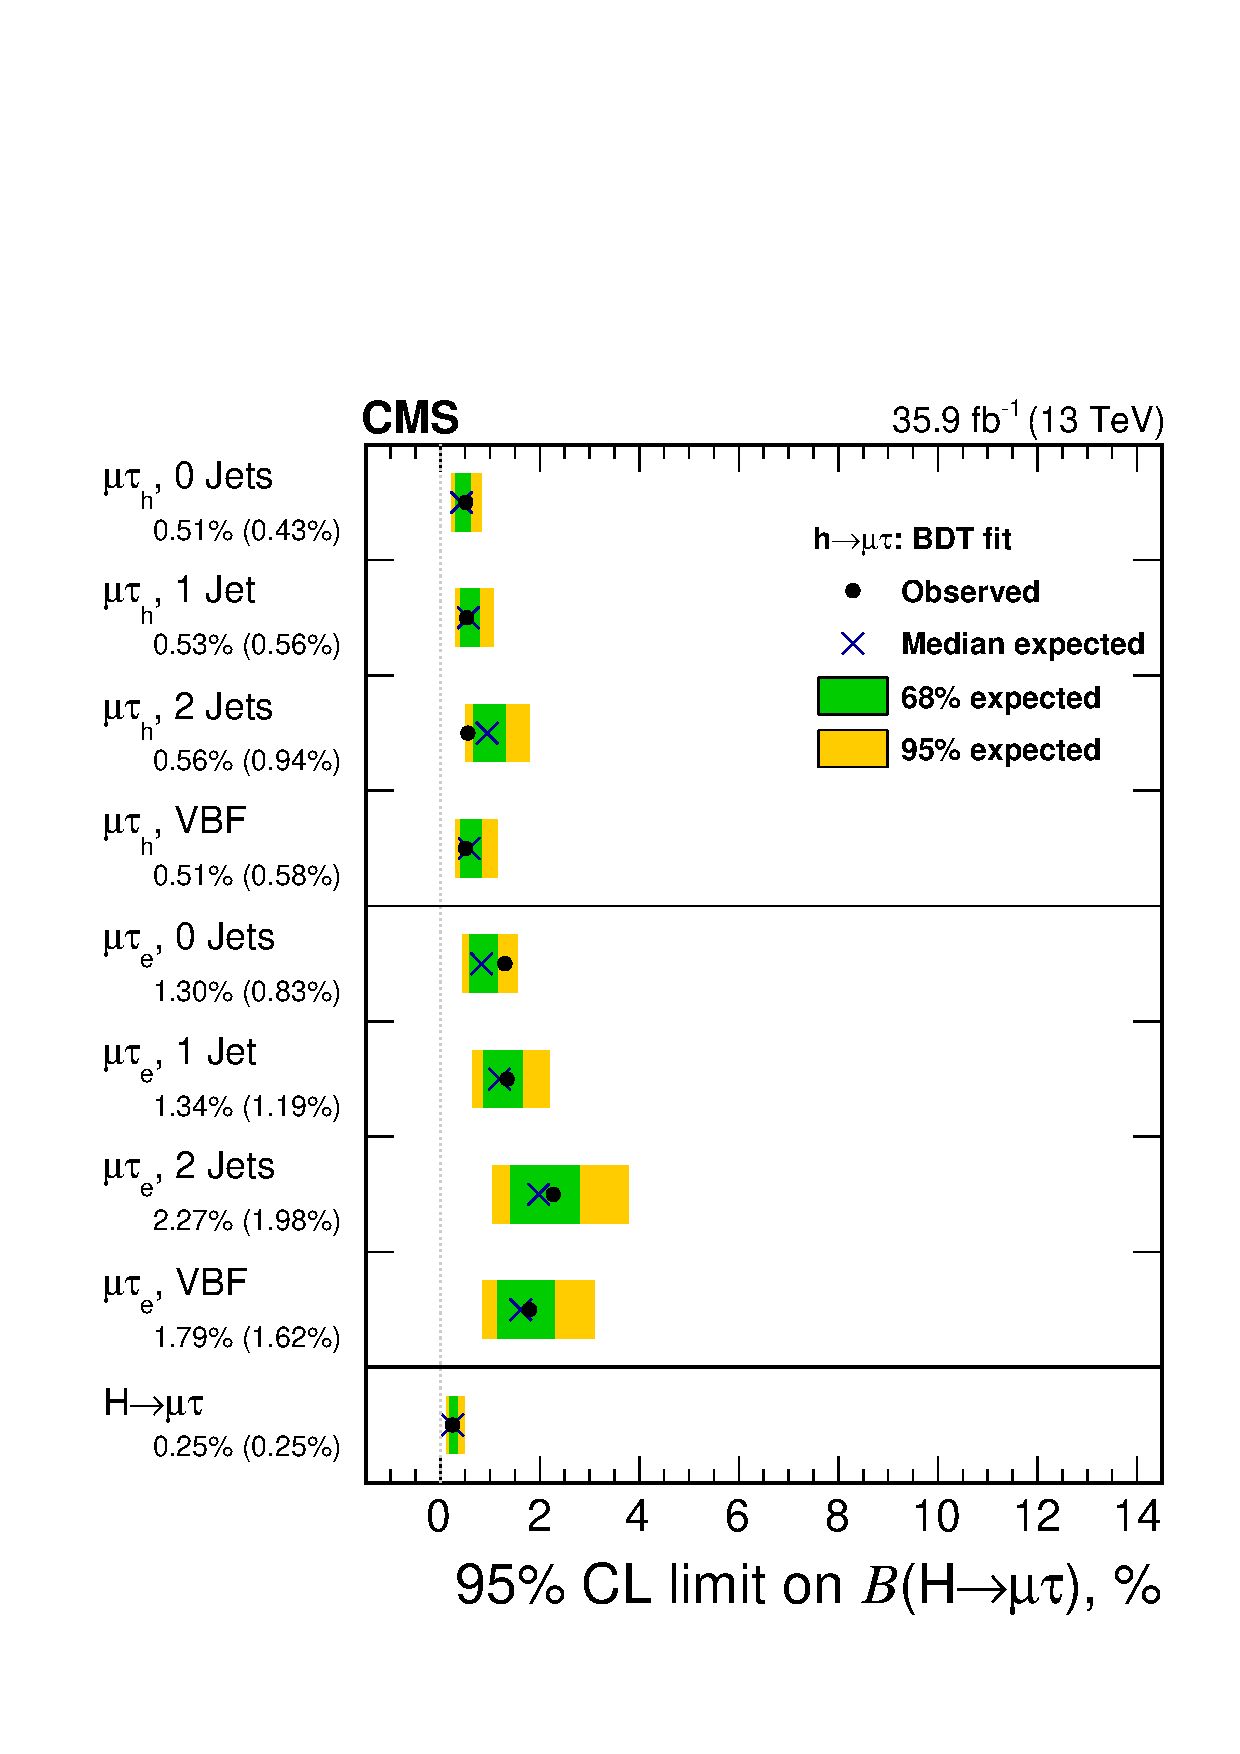
\includegraphics[width=0.49\textwidth]{plots_and_figures/chapter8/h125/brazilflagBDT.pdf}
 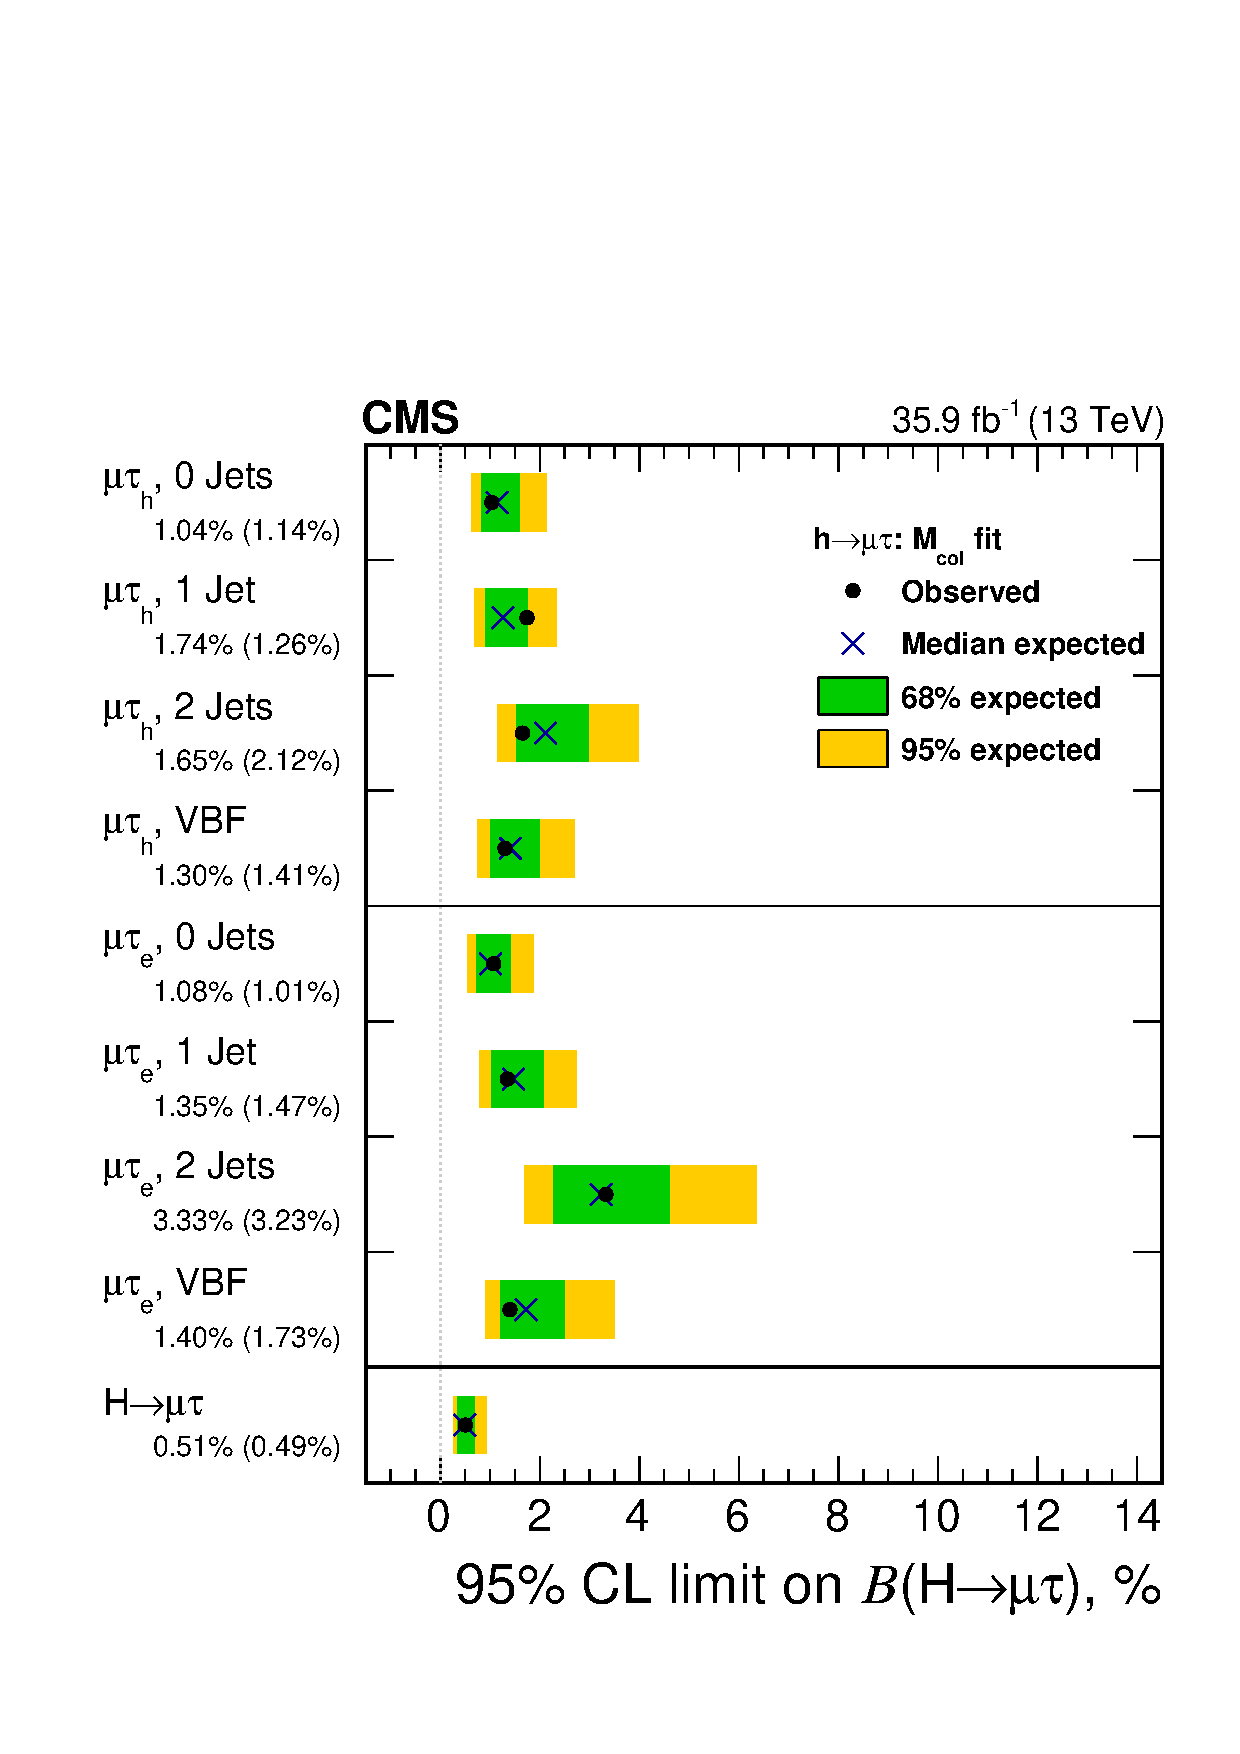
\includegraphics[width=0.49\textwidth]{plots_and_figures/chapter8/h125/brazilflagmcol.pdf} \\
 \caption{Observed and median expected upper exclusion limits for $\hmue$, $\hmuhad$ and combined $\hmu$ channels, for the BDT fit (left) and $\mcol$ fit analysis (right). The $\pm 1 \sigma$ and $\pm 2 \sigma$ bands for expected limits are also shown in light green and yellow respectively~\cite{HIG-17-001}.}
 \label{fig:hmue_limits_brazil}
\end{figure*}


The constraints on $\mathcal{B}(\hmu)$ can be transformed into constraints on Lepton Flavor Violating Yukawa Couplings ($Y_{\Pgm\Pgt},Y_{\Pgt\Pgm}$). These couplings represent the strength of an interaction and are related to the decay width $\Gamma(\hmu)$ in the following way~\cite{Harnik:2012pb}:
\begin{equation}                                                                                                                                                                                                 
\Gamma(\hmu)=\frac{m_{h}}{8\pi}(|Y_{\Pgm\Pgt}|^2 + |Y_{\Pgt\Pgm}|^2).                                                          
\label{eq:yuk1}
\end{equation}

The decay width is also related to the branching fraction, $\mathcal{B}(\hmu)$ according to the following equation:
\begin{equation}                                                                                                                                                                                                \mathcal{B}(\hmu)=\frac{\Gamma(\hmu)}{\Gamma(\hmu) + \Gamma_{SM}}.
\label{eq:yuk2}
\end{equation}

,where the SM Higgs decay width is assumed to be $\Gamma_{SM}=4.1$ MeV~\cite{Denner:2011mq} for $m_{\PH}=125$\GeV. Using equations~\ref{eq:yuk1} and ~\ref{eq:yuk2}, we derive the constraints on Yukawa couplings at 95\% CL. The limits for the Yukawa couplings are summarized in Table~\ref{table:yuk_coup}. Fig.~\ref{fig:yuk_coup} pictorially summarizes all existing limits on Yukawa couplings from different direct and indirect searches. It also shows the theoretical "naturalness" limit considering/expecting LFV couplings to be smaller than those of couplings for SM decays of the Higgs~\cite{Harnik:2012pb}, which can be considered a benchmark for sensitivity of this search. The limits derived from this search are most stringent till date, and surpass the above benchmark. 

\begin{table*}[!hbtp]
 \centering
  \caption{95\% CL observed upper limit on the Yukawa couplings,  for the BDT fit and the \mcol fit analysis.}
 \label{table:yuk_coup}
\begin{tabular}{|ccc| }
   \hline
                        & BDT fit  &  \mcol fit \\ \hline
$\sqrt{|Y_{\Pgm\Pgt}|^{2}+|Y_{\Pgt\Pgm}|^{2}}$   & $<1.43\times 10^{-3}$ &  $<2.05\times 10^{-3}$  \\
  \hline
\end{tabular}
\end{table*}

\begin{figure*}[!htpb]\centering
 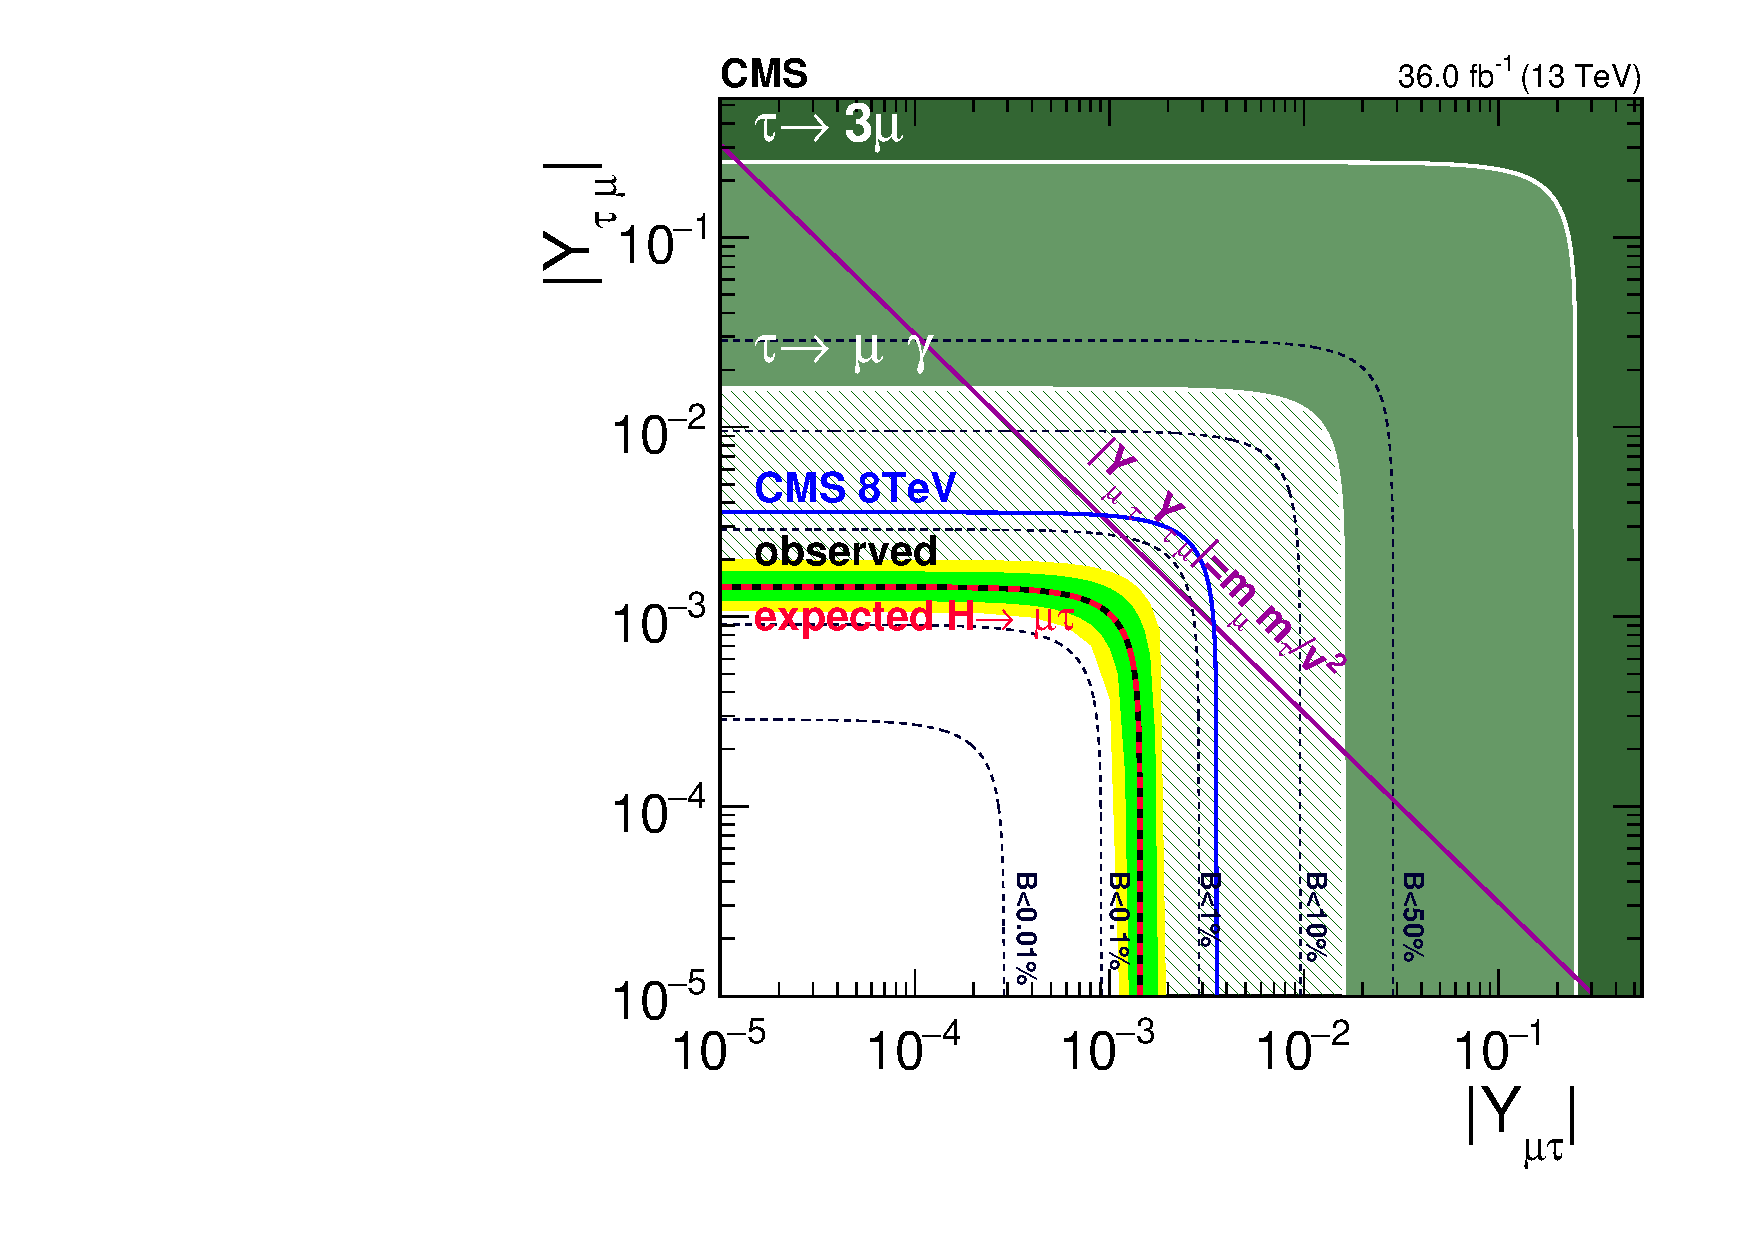
\includegraphics[width=0.6\textwidth]{plots_and_figures/chapter8/h125/yukawa.pdf}
 \caption{Observed (black solid)and median expected (red dashed) upper limits on $\hmu$ Yukawa couplings from this analysis. The light green and yellow bands show the $\pm 1 \sigma$ and $\pm 2 \sigma$ spreads of the expected limit. Blue solid line shows the result from the previous CMS search with 8 TeV data~\cite{Khachatryan:2015kon}. The naturalness limit is shown as a purple straight line.~\cite{HIG-17-001}}
 \label{fig:yuk_coup}
\end{figure*}


\subsection{$\Hmue$ results}
The resulting $\mcol$ distributions for signal and background estimation (after applying all selection requirements as outlined in ~\ref{HH_evt_sel}), after a binned maximum likelihood fit, are shown superimposed along with the observed data Fig~\ref{fig:mcol_dist_Hmue}. All systematic uncertainties are included as nuisance parameters, and the fit is performed simultaneously across all categories. We do not observe an excess over expected background in the entire range. Unlike the $\hmue$ analysis described above where the production cross-section of the SM Higgs boson is known, here we are looking for LFV decay of a hypothetical heavy Higgs bosons of different masses. Hence, we set upper exclusion limits on production cross-section times branching fraction, $\sigma(\textrm{gg}\rightarrow \PH)\times\mathcal{B}(\Hmue)$. The procedure is the same as used above and described in~\ref{exc_cal}. The observed and median expected upper limits at 95\% CL on $\sigma(\textrm{gg}\rightarrow \PH)\times\mathcal{B}(\Hmue)$ are summarized in table~\ref{table:limits_Hmue} for different categories and Higgs masses. The limits are also summarized graphically in Figure~\ref{fig:limits_Hmue}. The observed (median expected) limits range from 159.4 (95.6)\,pb to 2.9 (4.9)\,pb for heavy Higgs masses in the range between 200 and 900\,GeV. This search was combined with LFV heavy Higgs decay search with the tau lepton decaying hadronically, i.e. $\Hmuhad$ to produce constraints $\Hmu$. The combined observed (median expected) upper limits on $\sigma(\textrm{gg}\rightarrow \PH)\times\mathcal{B}(\Hmu)$ range from 51.9 (57.4)\,pb to 1.6 (2.1)\,pb. These limits are shown graphically in Figure~\ref{fig:limits_Hmu}. This is the first direct search till date to set limits on this decay.      

\begin{figure*}[!htpb]\centering
 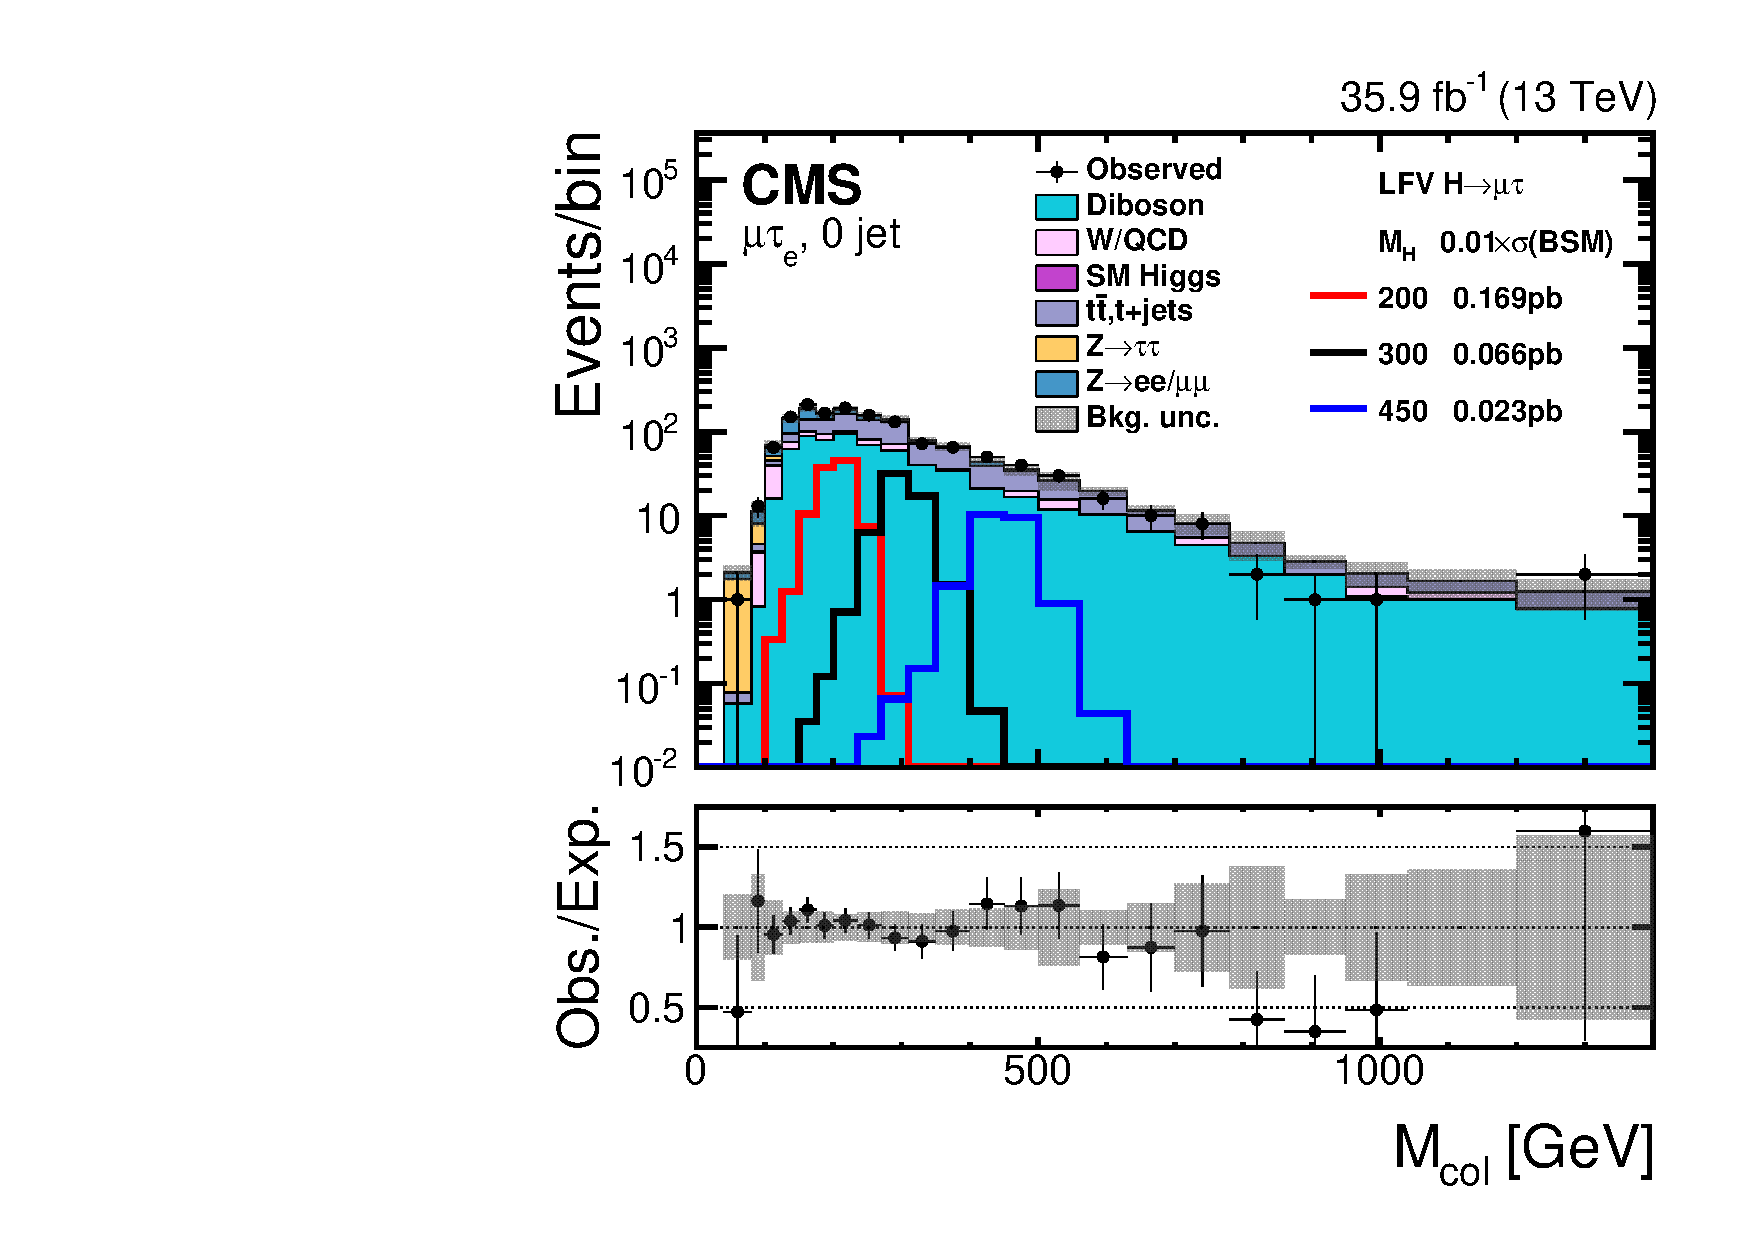
\includegraphics[width=0.49\textwidth]{plots_and_figures/chapter8/highmass/log_low_me_ch1_HMuTau_mutaue_1_2016_postfit_colmass_postfit.pdf}
 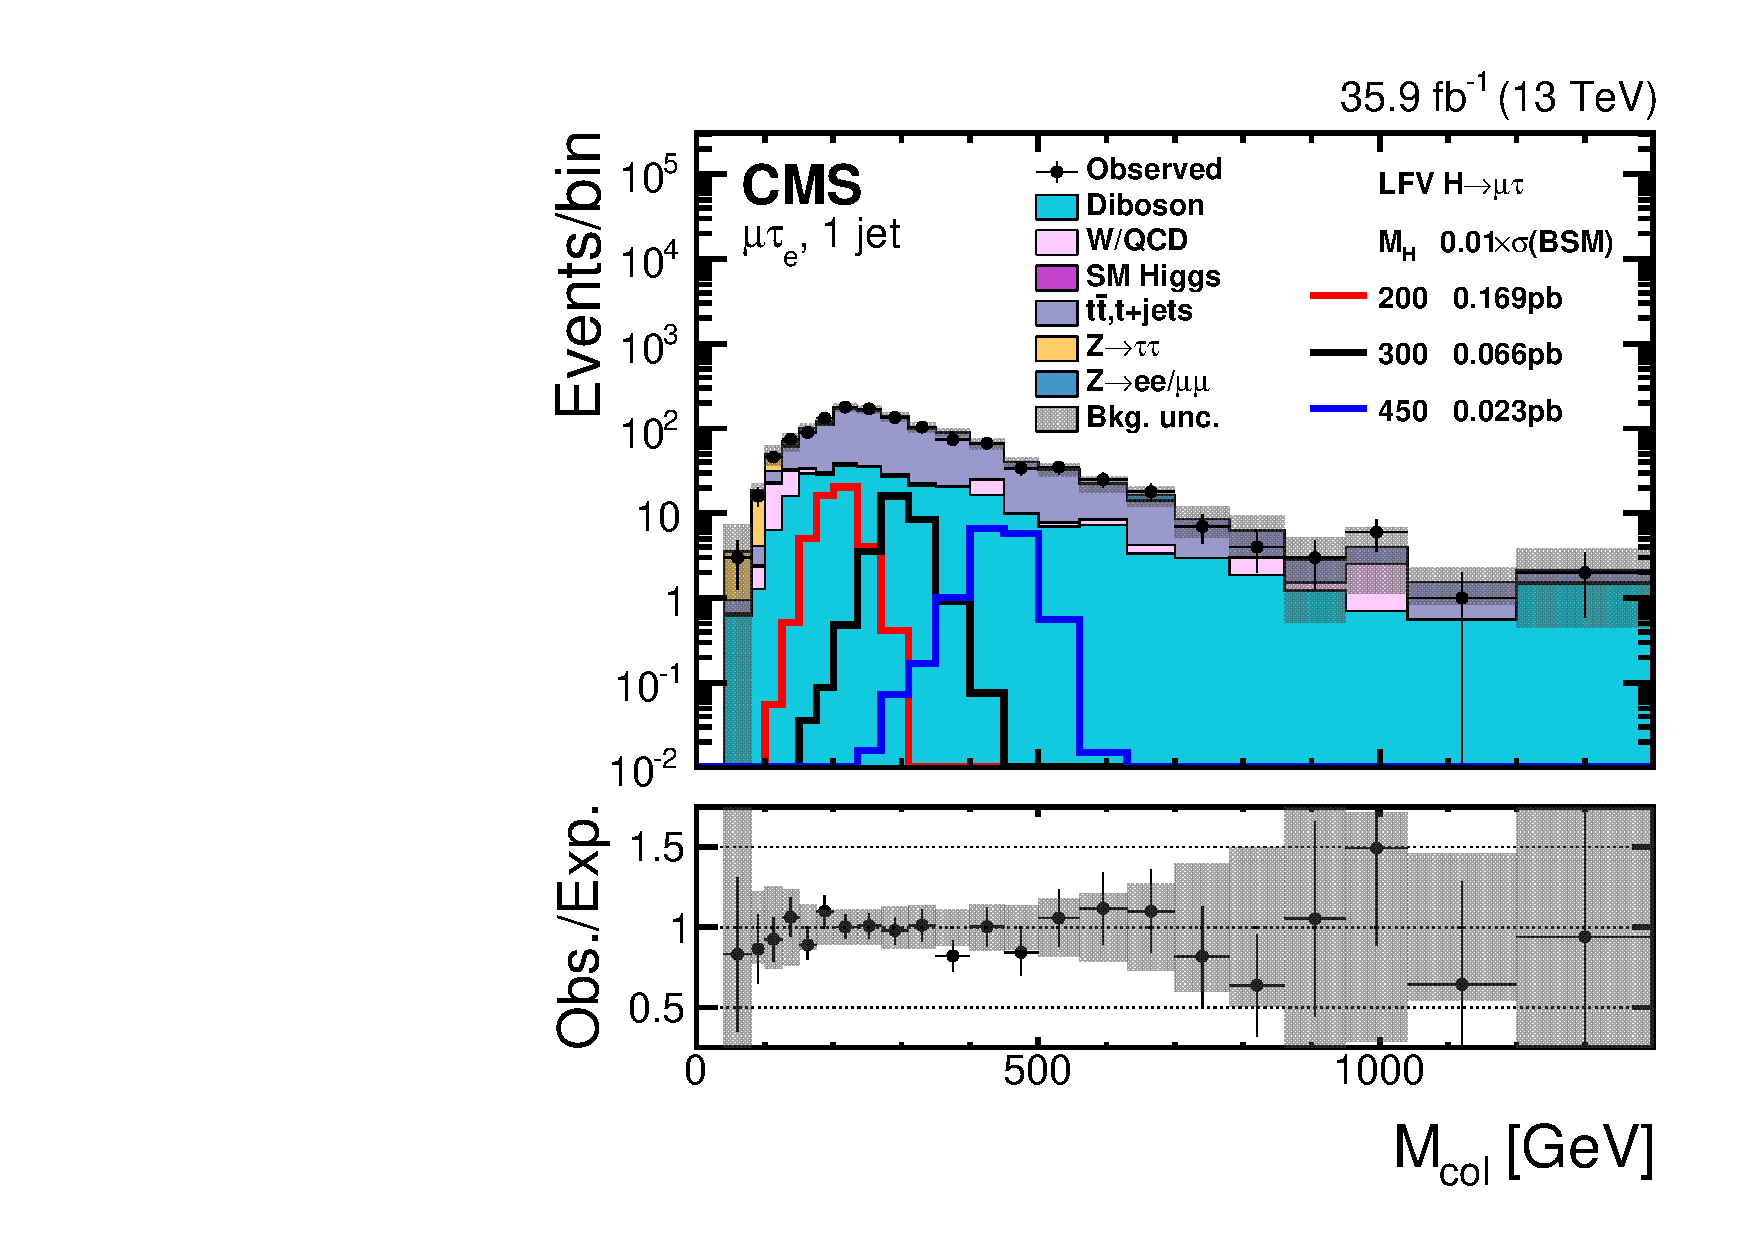
\includegraphics[width=0.49\textwidth]{plots_and_figures/chapter8/highmass/log_low_me_ch1_HMuTau_mutaue_2_2016_postfit_colmass_postfit.pdf} \\
 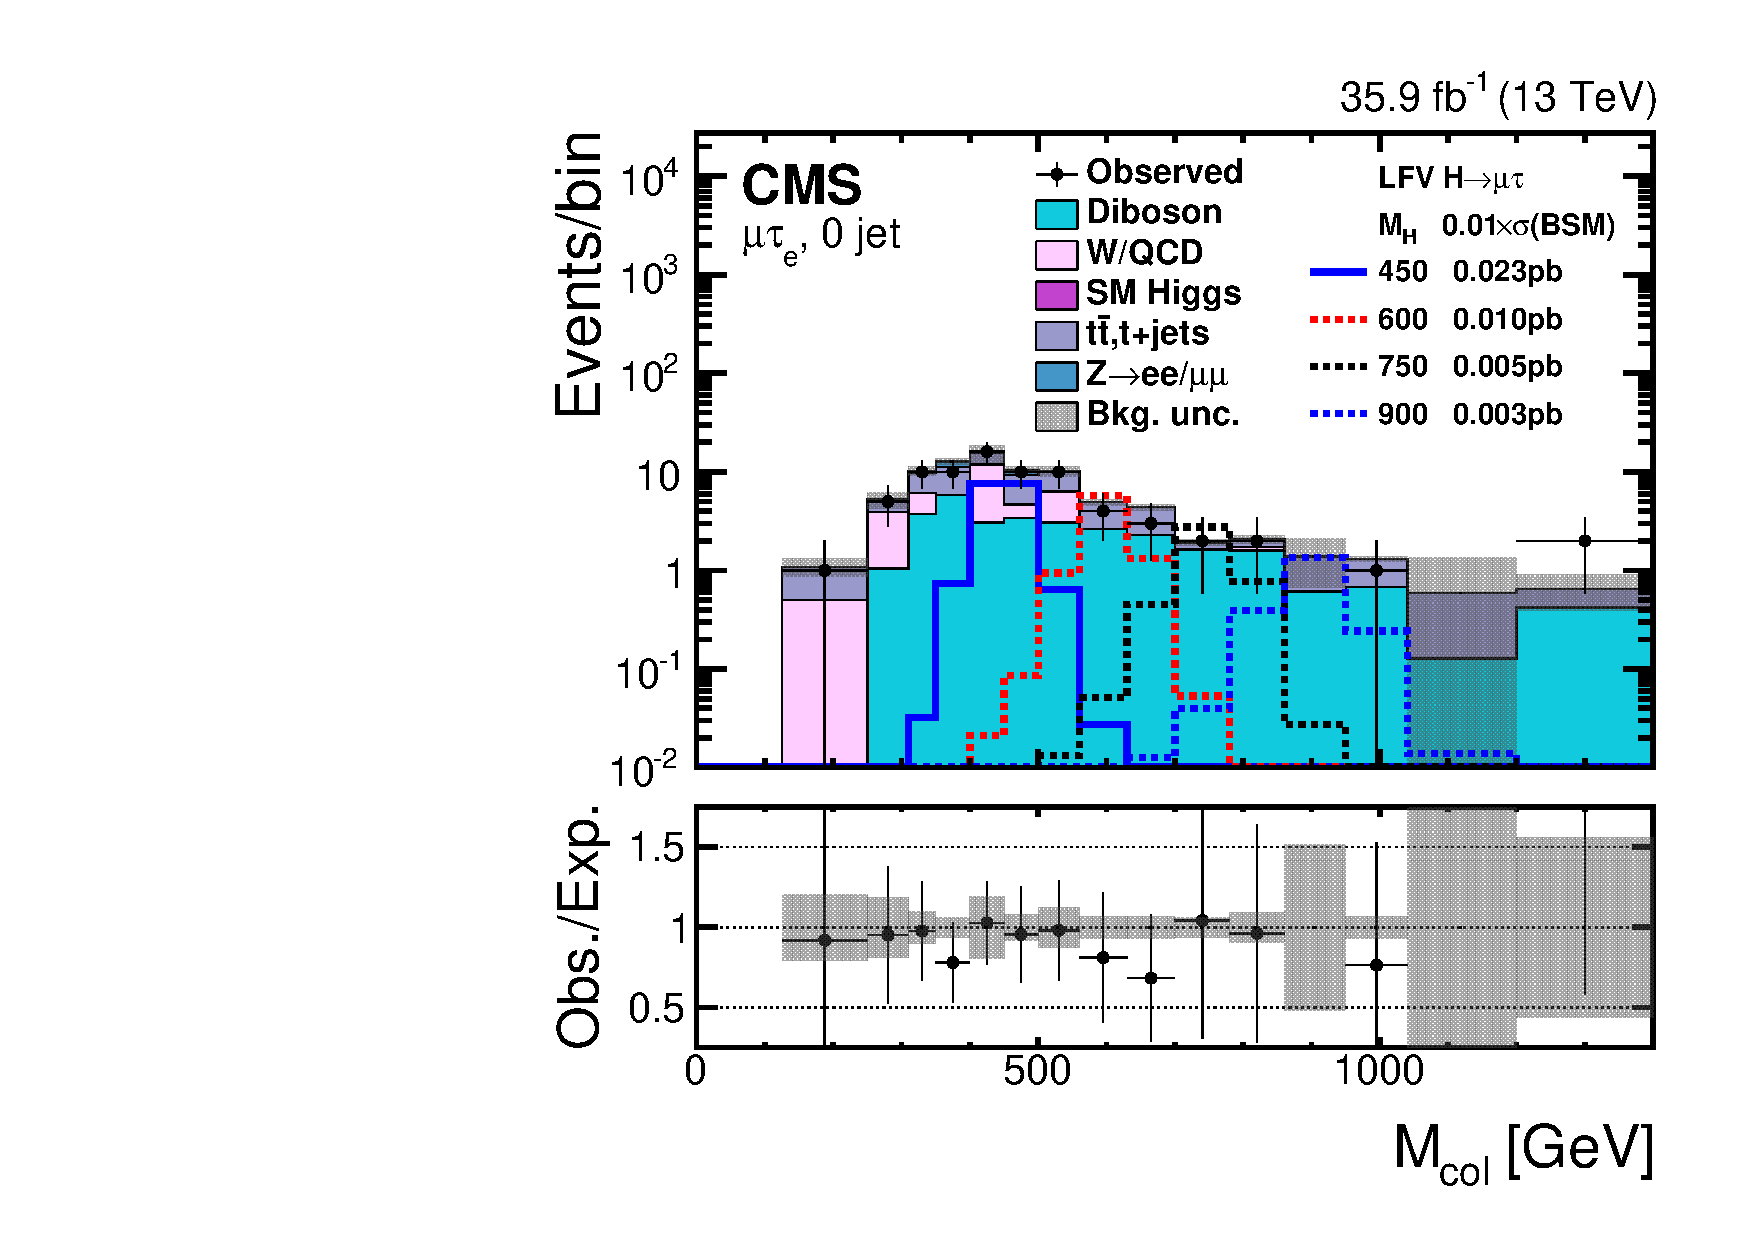
\includegraphics[width=0.49\textwidth]{plots_and_figures/chapter8/highmass/log_high_me_ch1_HMuTau_mutaue_1_2016_postfit_colmass_postfit.pdf}
 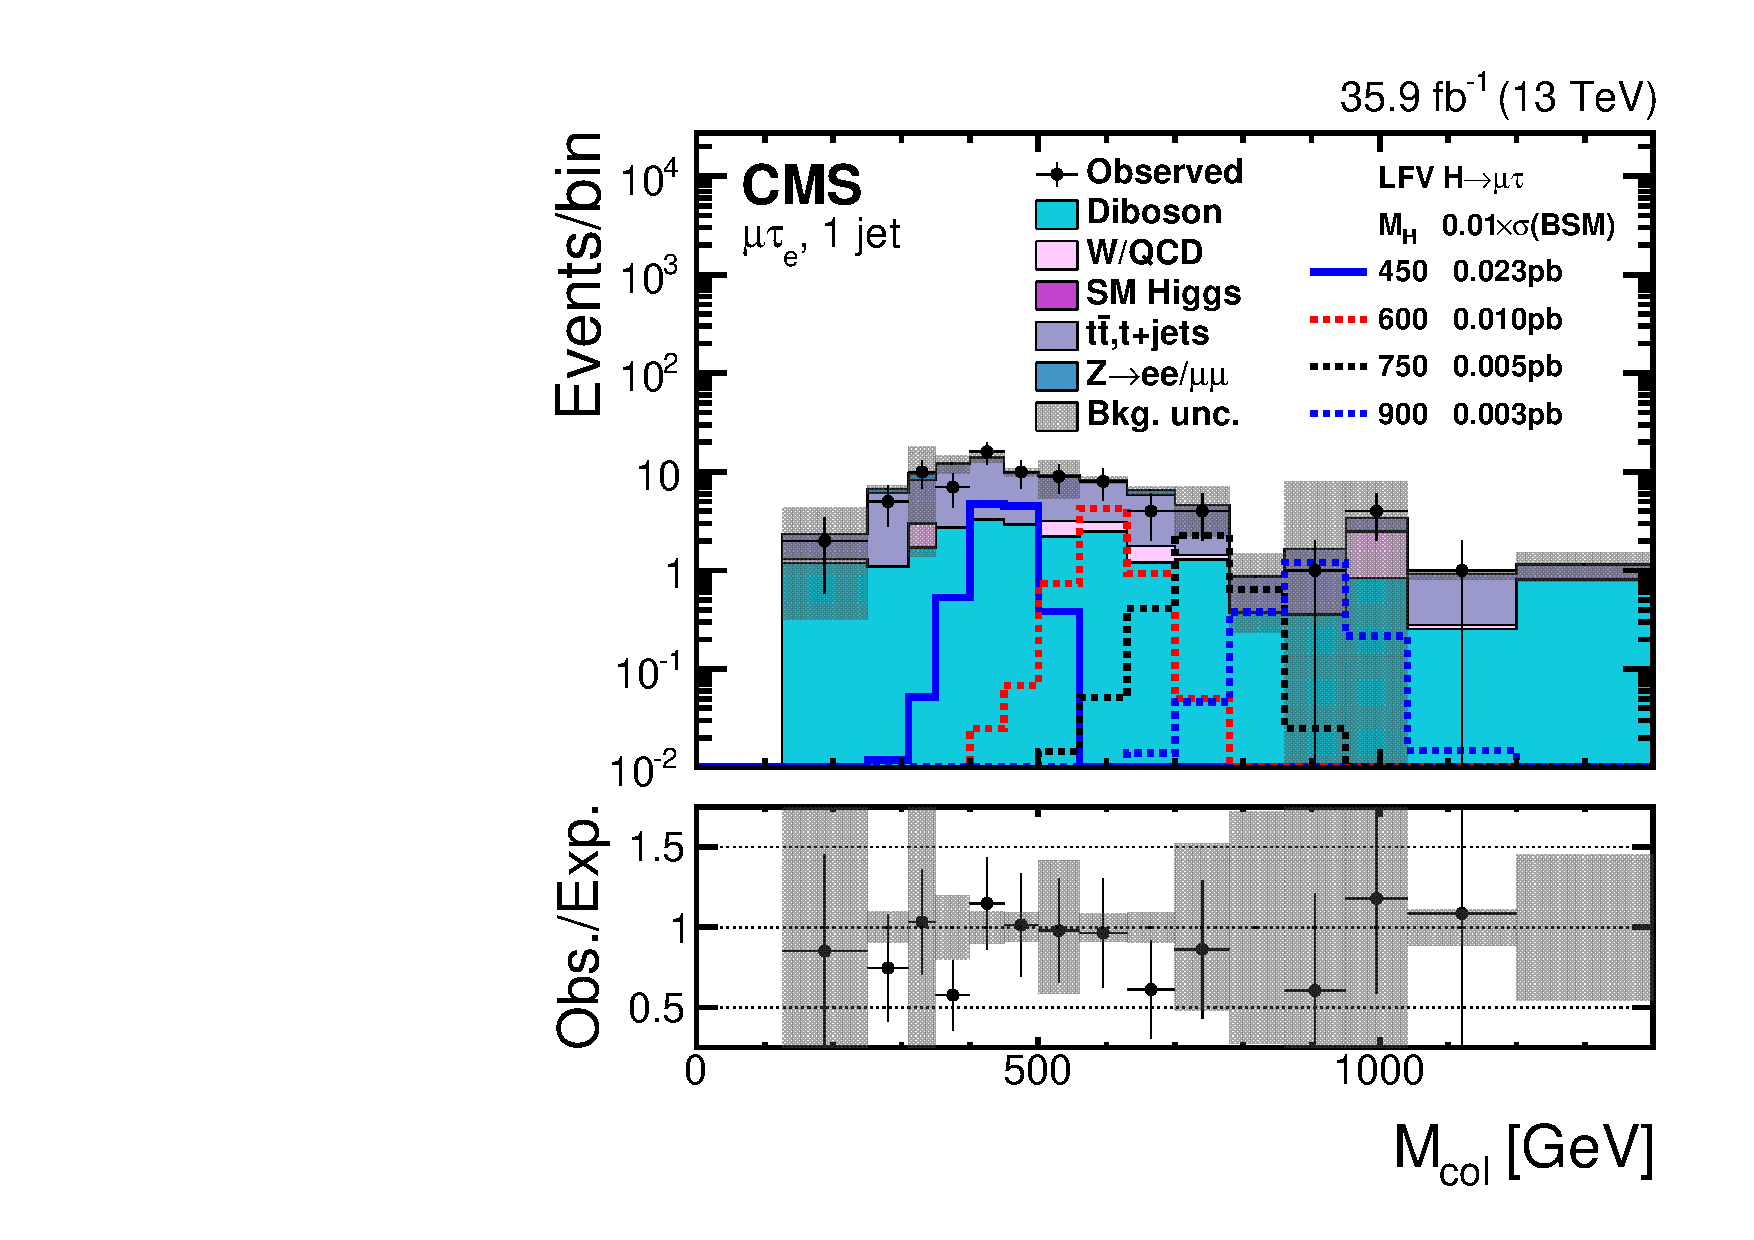
\includegraphics[width=0.49\textwidth]{plots_and_figures/chapter8/highmass/log_high_me_ch1_HMuTau_mutaue_2_2016_postfit_colmass_postfit.pdf} 
\caption{Distribution of $\mcol$ in 0-jet (left) and 1-jet (right) for lowmass (top) and highmass (range), comparing signal and background estimations to observed collision data, for $\Hmue$ analysis. The bottom panel show the ratio of observed data and fitted background in each bin~\cite{HIG-18-017}}
 \label{fig:mcol_dist_Hmue}
\end{figure*}


\begin{figure*}[!htpb]\centering
 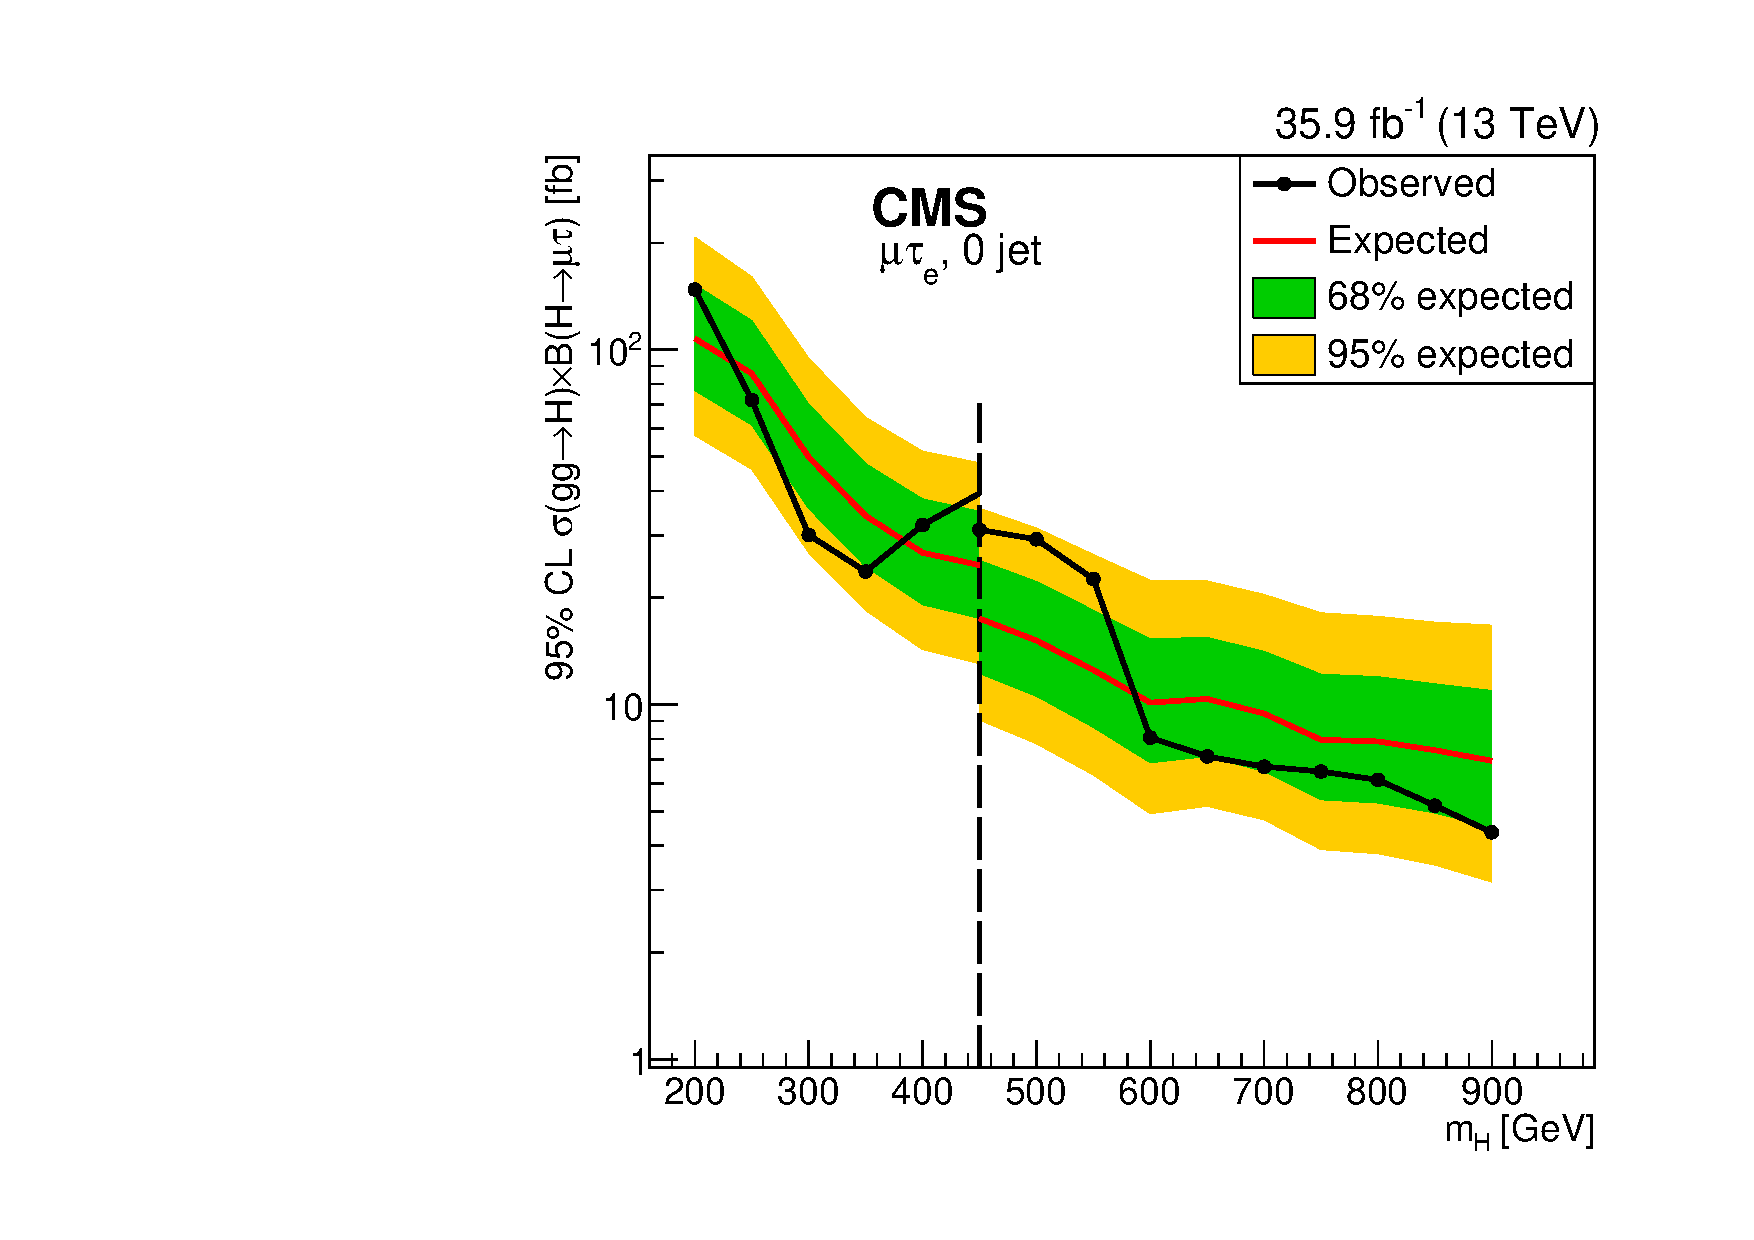
\includegraphics[width=0.49\textwidth]{plots_and_figures/chapter8/highmass/Figure_004-c.pdf}
 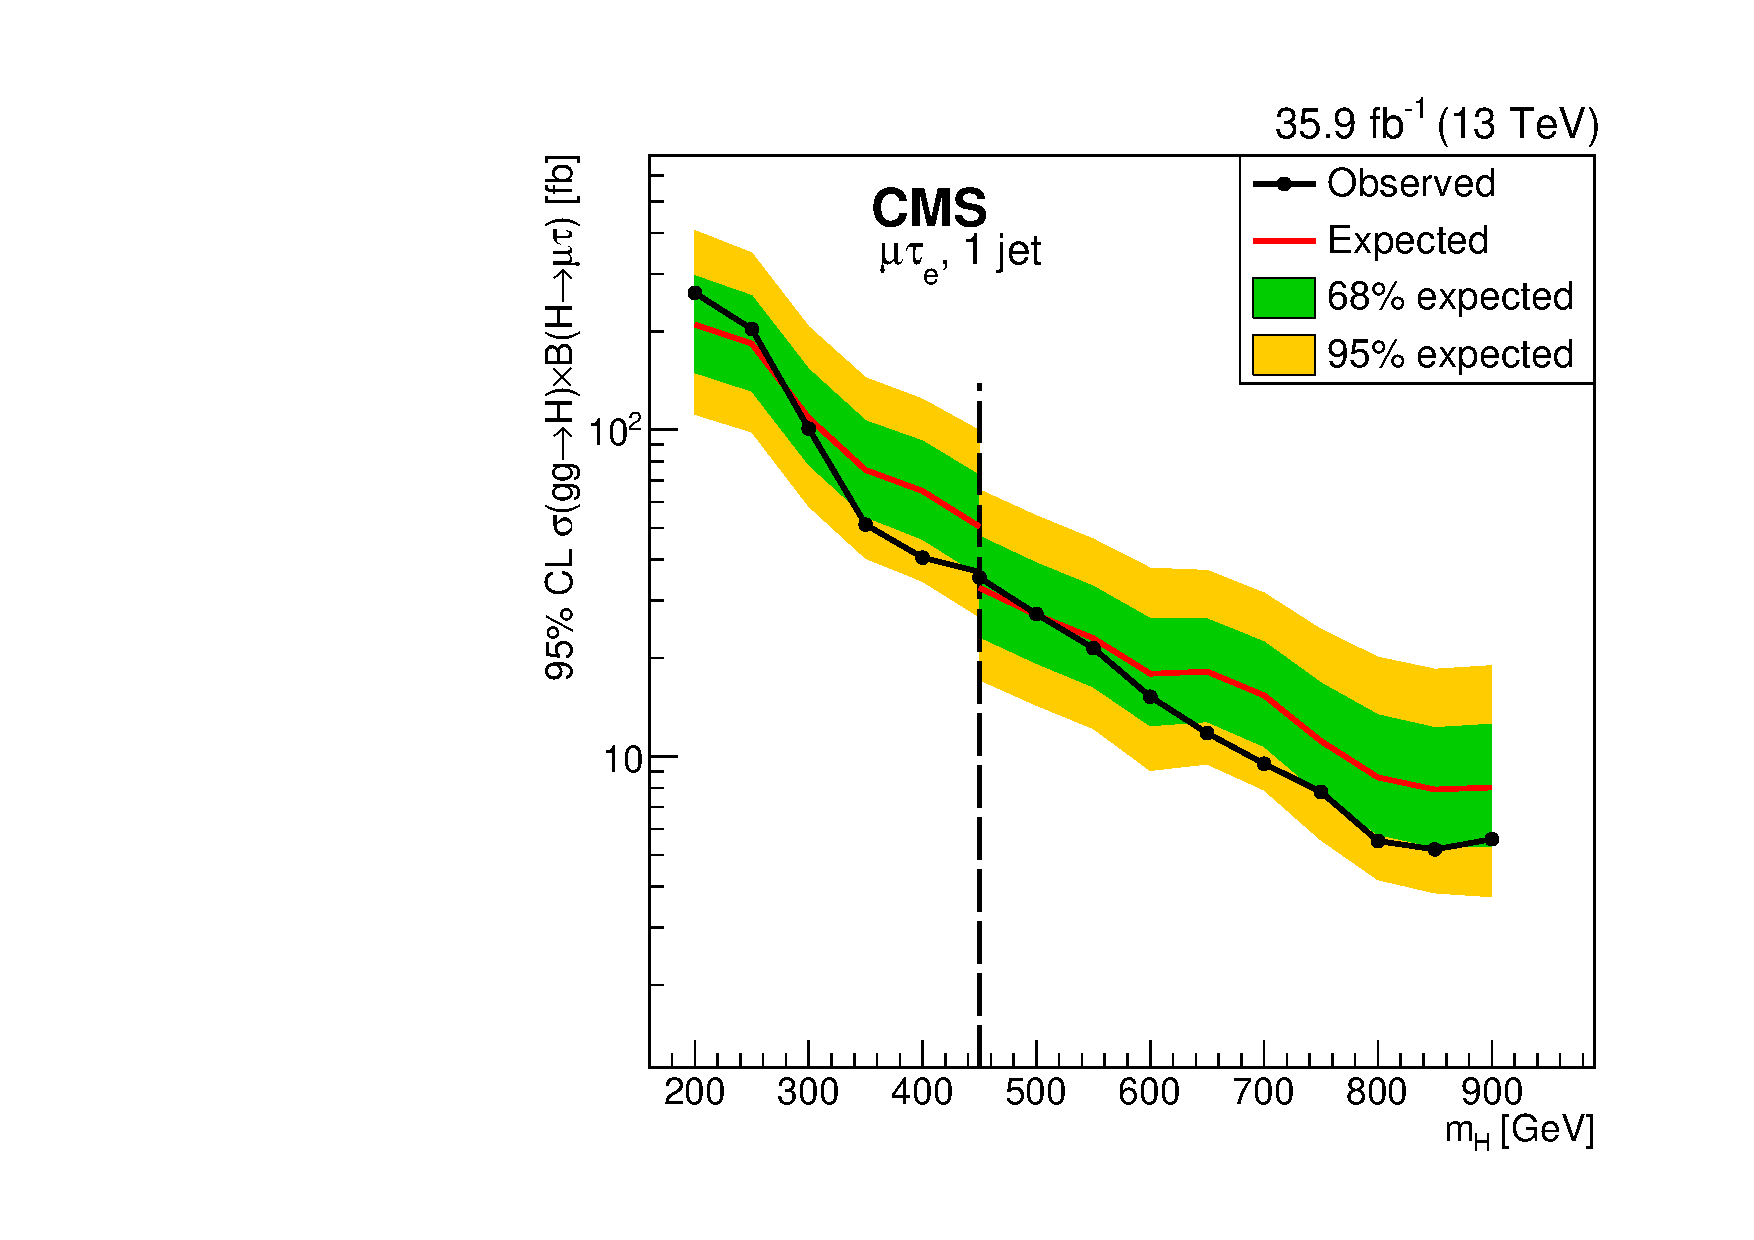
\includegraphics[width=0.49\textwidth]{plots_and_figures/chapter8/highmass/Figure_004-d.pdf} \\
 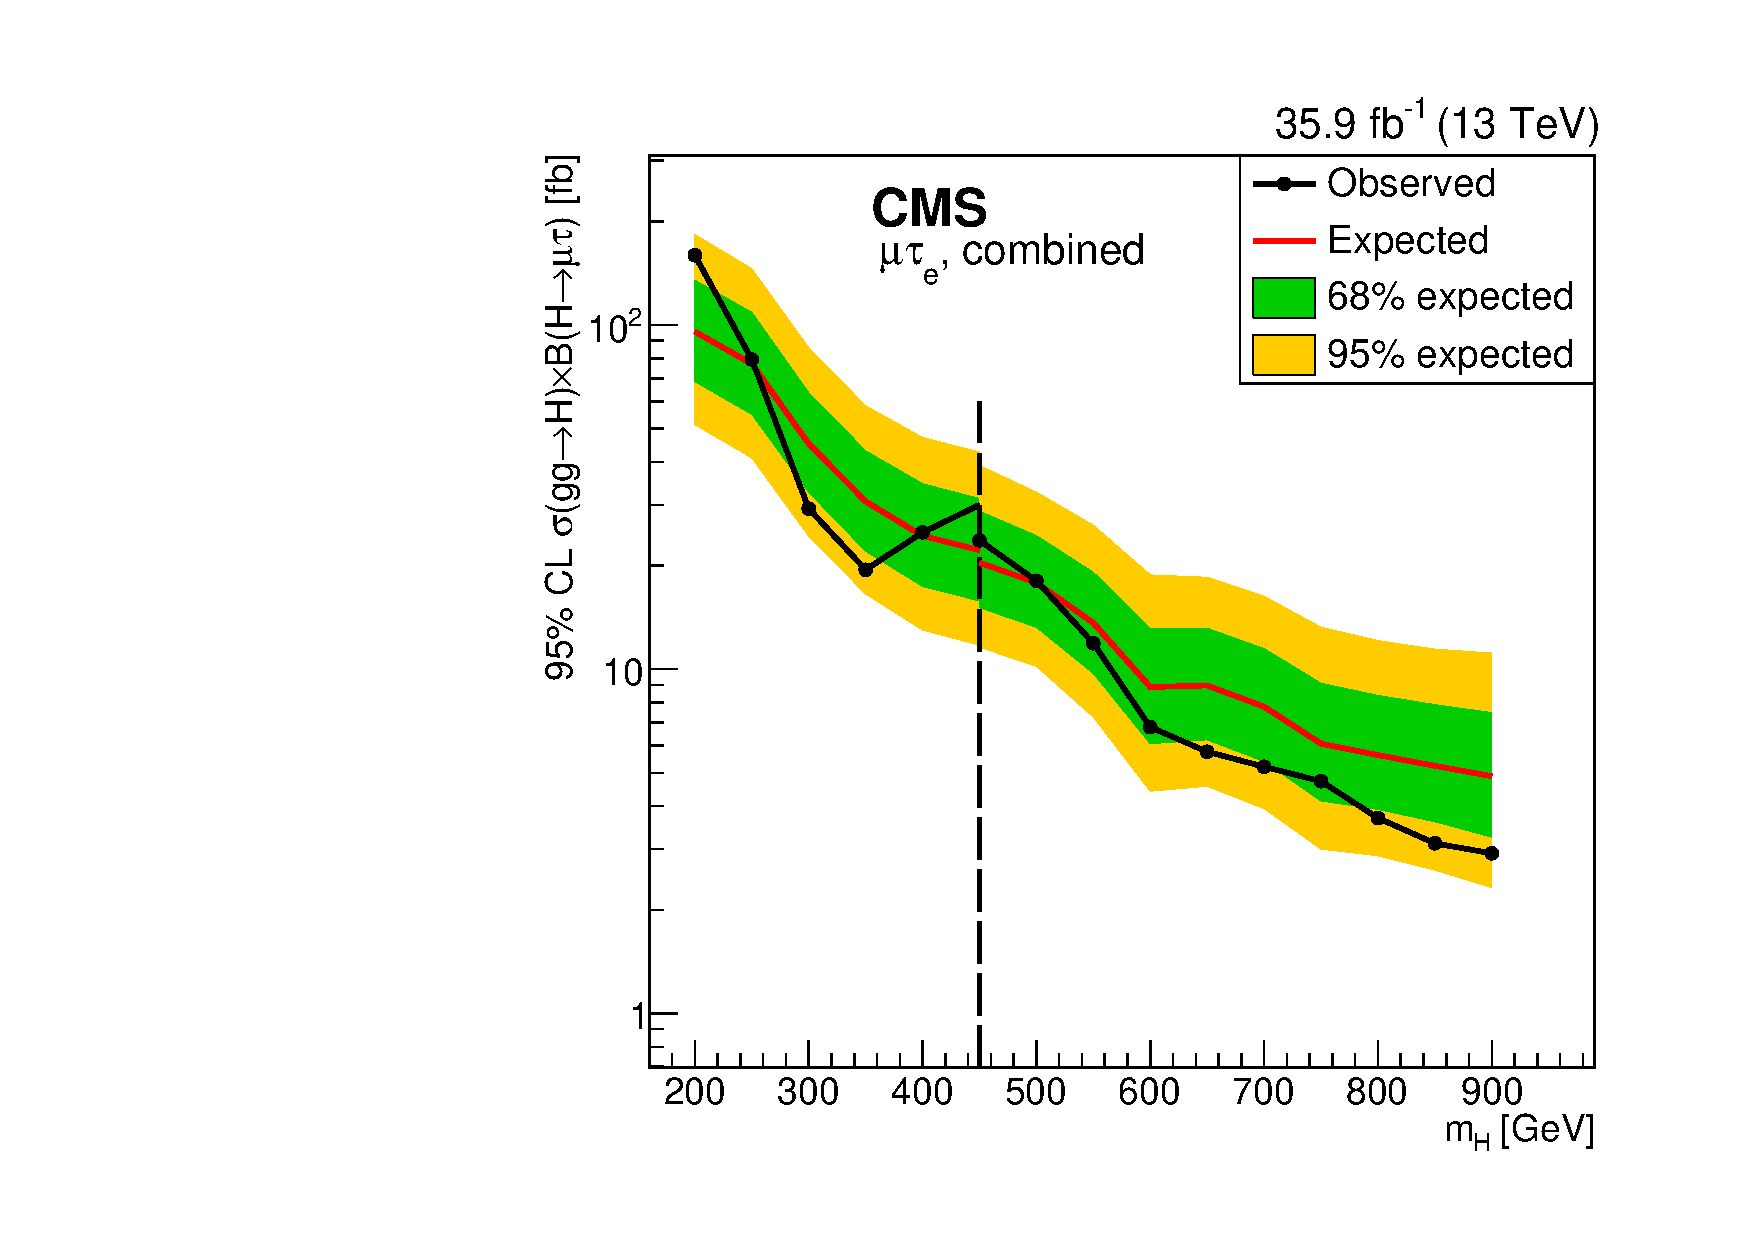
\includegraphics[width=0.60\textwidth]{plots_and_figures/chapter8/highmass/Figure_005-b.pdf}
\caption{Observed and Median expected 95\% upper exclusion limits for 0-jet (upper left), 1-jet (upper right) and combined (bottom),for the $\Hmue$ analysis. ~\cite{HIG-18-017}}
 \label{fig:limits_Hmue}
\end{figure*}



\begin{table*}
\caption{The observed (median expected) 95\% CL upper limits on $\sigma(\textrm{gg}\rightarrow \PH) \times\mathcal{B}(\Hmue)$.}
\begin{center}
\begin{tabular}{c|c|c|c}
\hline
$m_{\PH}$ (GeV) & 0 jet & 1 jet  & comb\\
\hline
200 &147.8 (107.5) & 262.1 (209.8)& 159.4 (95.6) \\
300 &30.1 (49.8) & 100.8 (108.6) & 29.3 (45.2) \\
450 &31.1 (17.5) & 35.3 (32.8) )& 23.7 (20.4) \\
600 &8.1 (10.4)& 15.2 (17.9)& 6.8 (8.9) \\
750 &6.5 (8.0)& 7.8 (18.2)& 4.7 (6.1) \\
900 &4.4 (6.9)& 5.6 (15.4)& 2.9 (4.9) \\
\hline
\end{tabular}
\label{table:limits_Hmue}
\end{center}
\end{table*}


\begin{figure*}[!htpb]\centering
 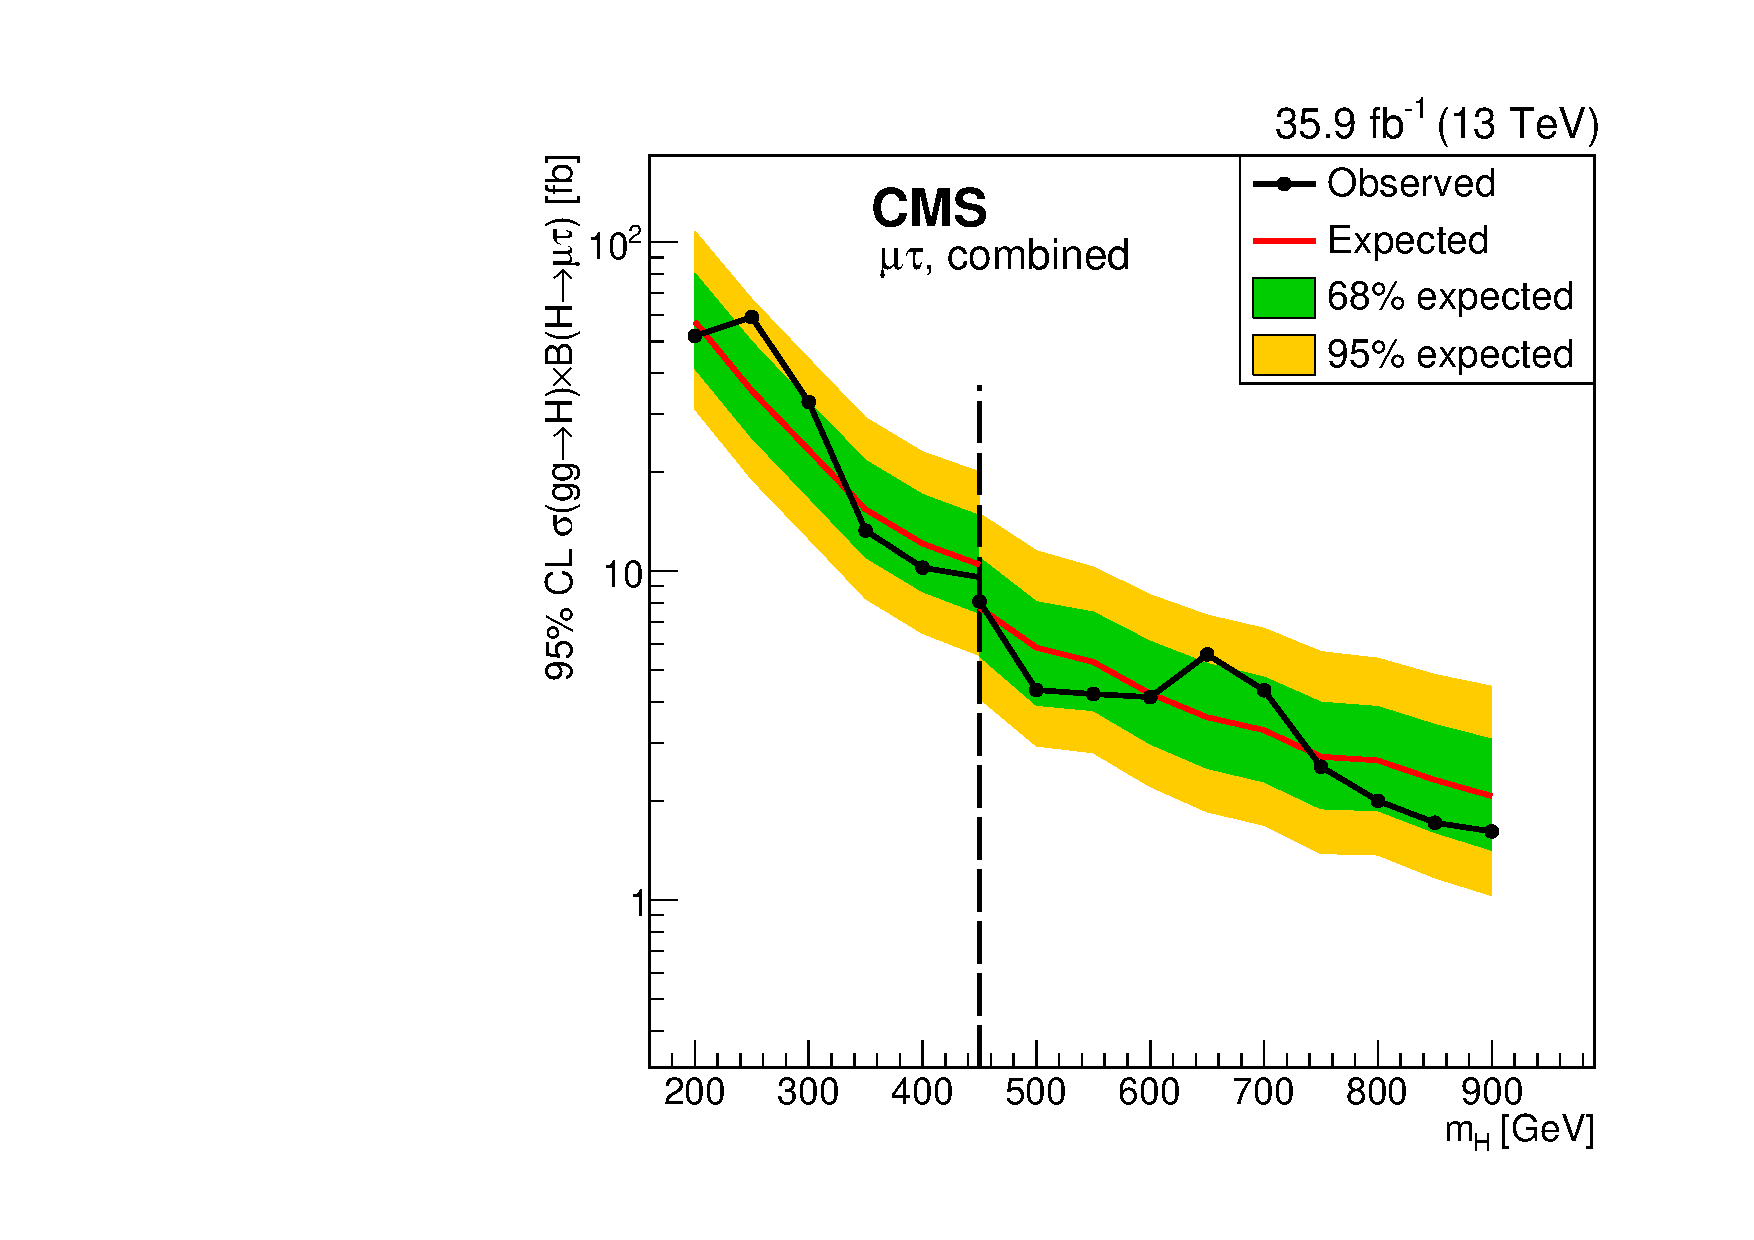
\includegraphics[width=0.8\textwidth]{plots_and_figures/chapter8/highmass/Figure_005-c.pdf}
\caption{Observed and Median expected 95\% upper exclusion limits for combined $\Hmu$ analysis~\cite{HIG-18-017}.}
 \label{fig:limits_Hmu}
\end{figure*}



% % uncomment the following lines,
% if using chapter-wise bibliography
%
% \bibliographystyle{ndnatbib}
% \bibliography{example}
